\documentclass[authoryear,review,11pt]{elsarticle}
\usepackage{lineno,hyperref}
\modulolinenumbers[2]
\usepackage[labelfont=bf]{caption}
\usepackage[dvipsnames]{xcolor}
\usepackage{amsmath}
\usepackage{amssymb,amsbsy,amsfonts}
\usepackage{soul} 
\usepackage[normalem]{ulem}
\usepackage{booktabs}
\usepackage{array,multirow}
\usepackage{changepage}
\usepackage{longtable}
\journal{Progress in Oceanography}

%%%%%%%%%%%%%%%%%%%%%%%%%%%%%%%%%%%%%%%%%%%%%%%%%%%
%% Elsevier bibliography styles
%%%%%%%%%%%%%%%%%%%%%%%%%%%%%%%%%%%%%%%%%%%%%%%%%%%%%%%%%

% Harvard
\bibliographystyle{elsarticle-harv}
\biboptions{authoryear}

%\newcommand{\digri}{\ensuremath{^{^\circ}}}
%\newcommand{\minute}{\ensuremath{^{^\prime}}}
\newcommand{\cdigri}{{\ensuremath{^{^\circ}}\mathrm{C}}}
\newcommand{\ndigri}{{\ensuremath{^{^\circ}}\mathrm{N}}}
%\newcommand{\sdigri}{{\ensuremath{^{^\circ}}\mathrm{S}}}
\newcommand{\edigri}{{\ensuremath{^{^\circ}}\mathrm{E}}}
\newcommand{\cms}{{\ensuremath{\mathrm{cm}~\mathrm{s}^{-1}}}}
\newcommand{\chla}{chl-{\emph{a}}}

% Title and Authors details
\begin{document}
\begin{frontmatter}

\title{Intraseasonal to interannual variability of zooplankton biomass and standing   stock inferred from ADCP backscatter in the eastern Arabian Seas}

%% Group authors per affiliation:


\author[1,2]{Ranjan Kumar Sahu}

\author[1,2]{D. Shankar\corref{cor1}}
\cortext[cor1]{Corresponding author}
\ead{shankar@nio.res.in}

\author[2,3]{P. Amol}
\author[1,2]{S.G. Aparna}
\author[1,2]{D.V. Desai}


\address[1]{CSIR-National Institute of Oceanography,Dona Paula,403004,Goa,India}

\address[2]{Academy of Scientific and Innovative Research (AcSIR), 
	Ghaziabad,
	201002,
	Uttar~Pradesh,
	India}

\address[3]{CSIR-NIO, Regional Centre, Visakhapatnam, 530017, Andhra Pradesh, India}

% **************************** Abstract *****************************


\begin{abstract}
	Variation of zooplankton biomass and standing stock in the eastern Arabian Sea (EAS) is mapped using backscatter measurements from 153.3~kHz acoustic Doppler current profiler moorings deployed at seven locations on the continental slope off the west coast of India from October 2017 to December 2023. The conversion from backscatter to biomass is based on volumetric zooplankton sampling. Zooplankton biomass in 24--140 m decreases from the upper ocean to lower depths. Changes are observed in seasonal variation of zooplankton standing stock monthly climatology (24--120 m biomass  integral) as we move poleward along the slope.  Standing stock variation is lowest at Kanyakumari followed by Okha, each at the southern and northern boundary of EAS, respectively. Annual cycle is predominant at northeastern Arabian Sea and it decreases towards southeastern Arabian Sea where the semi-annual cycle tends to dominate. The seasonal variation  Interannual variability, is observed with periods corresponding to $\sim$720 days, moderately off Mumbai and feebly off Goa. The use of seven moorings provides a map of variability along the slope from the southern end of EAS to almost its northern end.  Analysis reveals that the intraseasonal variation of zooplankton biomass is comparable to the seasonal variability which occurs within a season.	Stronger intraseasonal variability has implication on conventional sampling using ship-based methods because of the time it takes to cover EAS regime.
	
\end{abstract}

\begin{keyword}
	ADCP backscatter \sep zooplankton \sep biomass \sep standing stock \sep variability \sep eastern Arabian Sea
\end{keyword}
\end{frontmatter}


\pagebreak

% **************************** Main Text *****************************

\linenumbers

\section{Introduction}
\label{sec:intro}

\subsection{Background}
\label{sec:intro.back}

Zooplankton play a vital role in the food web of pelagic ecosystem by enabling the hierarchical transport of organic matter from primary producers to higher trophic levels, thereby impacting the fish population \citep{ohman2001density} and the carbon pump of the deep ocean \citep{le2016global}. They are presumably the largest migrating organisms in terms of biomass \citep{hays2003review} owing to their diel vertical migration (DVM). Zooplankton depend not only on phytoplankton, but also on the microbial loop \citep{azam1983microbial}; the zooplankton abundance or standing stock therefore depends on environmental variables (e.~g., mixed-layer depth or MLD, insolation, oxygen, thermocline, nutrient availability, Chlorophyll-\emph{a} (\chla) concentration, and daily primary production). As is true of the rest of the world ocean, the biological productivity of the north Indian Ocean (NIO; north of ~5$^{\circ}$N of Indian Ocean) is essentially driven by the physics and chemistry \citep[see, for example,][]{subrahmanyan1959studiespart2, banse1968hydrography, banse1995zooplankton, ryther1966primary, nair1970primary, qasim1977biological, levy2007basin, mccreary2009biophysical, vijith2016consequences, shankar2016inhibition, shankar2019role, amol2020modulation}, with changing dynamical conditions leading to variations in physico-chemical properties and therefore causing blooms and growth of plankton in favourable conditions. The changes are strongly influenced by the seasonal cycle in the NIO \citep{banse1968hydrography, mccreary1996four, mccreary2009biophysical, levy2007basin, shankar2019role, aparna2022seasonal}. The eastern boundary of the Arabian Sea contains the West India Coastal Current (WICC), which reverses seasonally, flowing poleward (equatorward) during November--February (June--September) \citep{banse1968hydrography, shetye1990hydrography, shetye19911517, vijith2022circulation, mccreary1993numerical, shankar1997dynamics, shankar2002monsoon}. 

%The eastern boundary of the Arabian Sea contains the West India Coastal Current \citep[WICC;][]{ramamirtham1965hydrography, banse1968hydrography, shetye1990hydrography, shetye19911517, mccreary1993numerical, shankar1997dynamics, shankar2002monsoon, amol2014observed, vijith2016consequences, chaudhuri2020observed}, which reverses seasonally, flowing poleward (equatorward) during November--February (June--September) \citep{shetye1990hydrography, shetye19911517, vijith2022circulation}.

A direct consequence of this reversal is the seasonal cycle of the thermocline \citep{shetye1990hydrography, shetye19911517, vijith2022circulation} and oxycline \citep{desousa1996seasonal, schmidt2020seasonal} due to the upwelling (downwelling) favourable conditions during summer (winter) in the eastern Arabian Sea \citep[EAS;][]{shetye1990hydrography, shetye19911517, vijith2022circulation}; the mixed-layer depth (MLD) responds to the changes in the thermocline and the mixing driven by the local winds and the changes in near-surface stratification \citep{shetye19911517, prasad1996mixed, prasannakumara20051848}. In response, the phytoplankton biomass and \chla\ concentration changes with season \citep{subrahmanyan1960studies, banse1968hydrography, prasannakumara20051848, levy2007basin, mccreary2009biophysical, vijith2016consequences, shankar2019role}. Upwelling during the summer monsoon leads to maximum \chla\ growth in the EAS \citep{banse1968hydrography, banse2000geographical, mccreary2009biophysical, hood2017biogeochemical, bemal2018picophytoplankton, shi2022phytoplankton}. During the winter monsoon, convective mixing driven by dry winds was considered the key process leading to the deep mixed layer in the northeastern Arabian Sea (NEAS) \citep{banse1968hydrography, shetye1992does, madhupratap1996mechanism, mccreary1996four, levy2007basin}, but recent results show that the poleward advection of warm and fresher water plays a key role in restricting the deep mixed layers to the northern part of the NEAS \citep{shankar2016inhibition}.  This deepening of the mixed layer leads to a winter \chla\ peak in the NEAS \citep{madhupratap1996mechanism, mccreary1996four, levy2007basin, shankar2016inhibition, vijith2016consequences, keerthi2017physical, shi2022phytoplankton}. In the southeastern Arabian Sea (SEAS), downwelling Rossby waves modulate \chla\ during the winter monsoon, but this effect is limited to the neighbourhood of the coast and islands \citep{amol2020modulation}; hence, the \chla\ peak in the SEAS is limited to the summer monsoon. 

The zooplankton grazing peak is instantaneous with no time delay from peak phytoplankton production \citep{li2000determines,barber2001qn}, but its population growth lags \citep{rehim2012dynamical, almen2020temperature} depending on its gestation period and other limiting aspects. Some studies suggest that the peak timing of zooplankton may not change in parallel with phytoplankton blooms \citep{winder2004climatic}, but others indicate that a lag exists between primary production and the transfer of energy to higher trophic levels \citep{brock1992interannual, brock1991phytoplankton}. Conventional, ship-based zooplankton sampling, which captures only a few snapshots of the variation, give an incoherent or incomplete understanding in terms of spatio-temporal variation of zooplankton \citep{ramamurthy1965studies, madhupratap1992zooplankton, piontkovski1995spatial, madhupratap1996lack, wishner1998mesozooplankton,nair1999arabian, barber2001qn, jyothibabu2010re, khandagale2022seasonal}. Generating a time series of zooplankton biomass and standing stock is, however, possible with calibrated acoustic instruments such as the acoustic Doppler current profiler (ADCP) \citep{edvardsen2003assessing, smith2005mesozooplankton, smeti2015spatial, kang2024acoustic}.  The ADCP, by providing a continuous time series at a high temporal resolution, can reveal details of the complex interplay between the physico-chemical and ecosystem variables \citep{jiang2007temporal, potiris2018acoustic, shankar2019role, aparna2022seasonal, nie2023influence}, and has been used to map zooplankton migration \citep{inoue2016diel,ursella2018evidence, ursella2021diel} and their seasonal to annual variation \citep{jiang2007temporal,  hobbs2021marine, liu2022seasonal, aparna2022seasonal}.

The relationship between ADCP backscatter and the abundance and size of zooplankton was described by \citet{greenlaw1979acoustical} with mono-frequency backscatter used to estimate abundance along with knowledge of mean zooplankton size. The popularity of the ADCP as a tool to study temporal and spatial variation of zooplankton biomass increased in the 1990s following the introduction of high-frequency echo sounders \citep{flagg1989use, wiebe1990sound, batchelder00981, greene1998three, rippeth1998diur}. The ADCP backscatter has been used to study DVM and the spatial and temporal variability of zooplankton biomass in different marine regions, such as the southwestern Pacific  \citep{smeti2015spatial}, the Lazarev Sea in Antarctica  \citep{cisewski2010seasonal}, the Canadian Arctic  \citep{hamilton2013links}, and the Corsica Channel in the northwestern Mediterranean Sea \citep{guerra2019zooplankton}. With networks of moored buoys deployed across the world ocean to measure currents, the potential use of acoustics for understanding coupled physical and biological processes is, however, yet to be fully exploited \citep{davis2019100}. The first such study to explore the potential of ADCPs in EAS was carried out by \citet{aparna2022seasonal} (A22 hereafter) using ADCP moorings deployed on continental slope off the Indian west coast. 

\subsection{Objectives and scope}
\label{sec:intro.scope}

The network of ADCPs used by A22 to map the seasonal cycle of zooplankton biomass and standing stock was originally deployed on the continental slope off the west coast of India to map the variability of the WICC on time scales ranging from the seasonal to the intraseasonal and to provide a measure of its interannual variability \citep{amol2014observed, chaudhuri2020observed}. A22 showed that the zooplankton peaks (and troughs) are influenced by the the seasonal movement of the thermocline, the oxygen minimum zone (OMZ), and the MLD. Their analysis showed that the zooplankton standing stock (ZSS) tends to decrease in the SEAS during the summer monsoon, when upwelling facilitates an increase in phytoplankton biomass.

A22 used ADCP backscatter data from three moorings, one each located off Mumbai (NEAS), Goa (central-eastern Arabian Sea or CEAS), and Kollam (SEAS).  We extend the work of A22 by presenting data from four additional moorings in the EAS and highlight the significant intraseasonal variability of biomass and standing stock revealed by the ADCP data. The article is organized as follows: datasets and methods employed are described in section~\ref{sec:data}. Section~\ref{sec:seasonal} describes the observed time series and the climatology of zooplankton biomass and standing stock and their seasonal cycle and variability. A brief discussion on interannual variability in section~\ref{sec:interannual} is followed by a detailed discussion in section~\ref{sec:intraseasonal} on intraseasonal variability, which is a major focus in this study. Section~\ref{sec:discuss} summarises the results and discusses their implications.


\section{Data and methods}
\label{sec:data}

In this section, we describe the data sets used in this article: the primary data are ADCP backscatter (section~\ref{sec:data.bs}) and zooplankton biomass (section~\ref{sec:data.biomass}), but we also use data on temperature, salinity, MLD, oxygen, and \chla\ (section~\ref{sec:data.misc}).

\subsection{The ADCP backscatter time series}
\label{sec:data.bs}

The ADCP backscatter forms the primary data set used in this article.  The four additional moorings include one off Kanyakumari (in the SEAS, south of Kollam and on the slope off the southern tip of the Indian mainland), Udupi (just north of the SEAS--CEAS boundary), Jaigarh (north of Goa in the CEAS), and Okha (north of Mumbai in the NEAS); all these mooring locations are shown in Fig.~\ref{fig:map} and listed in Table~\ref{tab:moorings}.  The ADCPs are of make Teledyne RD Instruments, upward-looking, and operate at 153.3~kHz.  Though the Kanyakumari mooring had been deployed in 2009, the top ADCP had a frequency of 76.8~kHz till January~2016, over two years after the shift to 153.3~kHz off Kollam, Goa, and Mumbai  \citep{chaudhuri2020observed}.  That's why the Kanyakumari mooring was not included in the analysis of A22.  We include it in our analysis because it starts in October~2017, when the other three moorings were deployed in the EAS.

The moorings on the west-coast slope are serviced once a year during September--December depending on ship availability. Data was collected at hourly intervals with a 4~m bin size. The echoes at the surface render the data useless within roughly 10\% of the transducer's range ($\sim$20~m) and this data is therefore discarded.  We have followed the methodology laid down in A22 to derive the backscatter time series from ADCP echo intensity. Gaps up to two days are filled using the grafting method of \citet{mukhopadhyay2017st} and the graft-filled backscatter time series is converted to zooplankton biomass.

%ADCPs were deployed on the continental slope off the Indian west coast (Fig.~\ref{fig:map}), off Mumbai, Goa, and Kollam, and later extended to an additional four sites to cover the entire EAS basin from Okha (22.26$^{\circ}$N) in north to Kanyakumari (6.96$^{\circ}$N) in south. The other two ADCPs are 1) Jaigarh at central EAS (CEAS) and 2) Udupi (primarily at SEAS regime) in the transition zone between CEAS and SEAS. The extended moorings were deployed in October 2017, though Kanyakumari had been deployed earlier. The moorings are serviced on a yearly basis, usually during October--November or sometime during September--December (depending on ship availability). The ADCPs are of Teledyne RD Instruments  make, upward-looking and operate at 153.3 kHz. While utmost care is taken to position the instrument (mooring) at  $\sim$150--200 m ($\sim$1050-1100 m) depth, yet for some deployments it's shallower or deeper owing to drift caused by floater-buoyancy and anchor-weight imbalance. Data was collected at hourly intervals with a 4 m bin size. The echoes at surface to 10\% range ($\sim$20 m) render the data useless and is discarded from further use.  We have followed the methodology laid down in A22 to derive the backscatter time series from ADCP echo intensity. Gaps up to two days are filled using the grafting method of \citet{mukhopadhyay2017st}. Graft-filled backscatter time series is converted to zooplankton biomass.


\subsection{The zooplankton biomass time series}
\label{sec:data.biomass}

In situ biomass data from volumetric zooplankton samples are used to convert the backscatter to biomass.  The zooplankton  samples were collected in the vicinity ($\sim$10~km) of the ADCP mooring site twice, once prior to retrieval and again following the deployment of the mooring (table~\ref{tab:mpn}). A multi-plankton net (MPN, 100~$\mu$m mesh size, 0.5~m$^2$ mouth area) was used to collect samples in the pre-determined depth ranges; the water volume filtered was calculated by sampling depth range and mouth area.  The timing of sample collection was different throughout the MPN hauls owing to its dependence on the time or mooring retrieval, but the depth range was standardized from 2020 onwards to the bins over 0--25, 25--50, 50--75, 75--100, and 100--150~m. Following numerous previous studies \citep[A22;][]{flagg1989use, heywood1991estimation, jiang2007temporal}, the backscatter was averaged in the vertical corresponding to the specific bins of MPN haul for each site and then linearly regressed with the biomass of respective bins (Fig.~\ref{fig:bstobm}). The zooplankton biomass in the euphotic zone concentrates in the upper 10~m and this shift to near the surface is pronounced during the night. Yet, this should not be a concern for the regression as it would simply show up as low backscatter at deeper depths during night-time corresponding to low biomass. It is important to note that the study is carried out using daily averaged biomass. Therefore, features associated with DVM are eliminated \citep[A22;][]{jiang2007temporal}.

%\subsubsection{Biomass time series and estimation of standing stock}
%\label{sec:data.biomasstimeseries}

The zooplankton biomass time series (Fig.~\ref{fig:biomass_daily_monthly}) is created from the above linear regression. The standing stock is determined by taking the vertical integral of biomass over the water column. As in A2, to maintain consistency in the estimation of standing stock over the time series, only those deployments that do not lack data at any depth in the entire range of 24--120 m are considered for analysis. The lack of data above $\sim$24~m is due to the deviation in the vertical position of the ADCP transducer in the water column. In spite of the care taken to position the instrument (mooring) at  $\sim$150--200~m ($\sim$1050--1100~m) depth, the process of mooring deployment, which is done from a steaming ship, implies that some deployments are shallower or deeper owing to drift caused by floater-buoyancy and anchor-weight imbalance. It leads to a gap in the data at some mooring sites for some years. For example, off Okha, data is not available for the entire upper 120~m depth for the second deployment (2018--2019). Data is also unavailable off Jaigarh from the surface to $\sim$60~m data during 2019--2022 and off Kollam during 2020--2021 below $\sim$80~m. There are also a few deployments during which no data or bad data was recorded, e.~g, off Udupi (2020--2021) and Kanyakumari (2022--2023); such bad data are discarded from standing-stock estimation. 	

A decrease in biomass with increasing depth is observed at all seven locations (Fig.~\ref{fig:biomass_daily_monthly}).  To demarcate this expected decrease in biomass from the more productive upper ocean to the less productive lower ocean, A22 used the 215~mg~m$^{-3}$ biomass contour (called $z215$), and this contour is plotted for both daily and monthly time series in Fig.~\ref{fig:biomass_daily_monthly}; the depth of this contour is called $D215$.  The lower biomass in the upper ocean off Kanyakumari and Okha, however, led us to use the 175~mg~m$^{-3}$ for these locations.  This contour, whether $D215$ or $D175$, cannot be plotted when data are missing, leading to some gaps in its time series.  

%More striking, however, is the missing contour off Kollam in 2020: the biomass here was unusually low during 2020, leading to the contour being missing over the entire year.

%To distinguish between high and low productivity zones, we employed a biomass contour similar to the 215 mg~m$^{-3}$ threshold used in A22, but with the exception of Kollam during 2020, as variation in the monthly averaged data suggests presence of strong interannual variability. It is of two distinct types: 1) deviation from the seasonal cycle which is aperiodic, 2)~variation associated with interannual climate modes, which is quasi-periodic. For the years 2019 and 2020 the low biomass is observed at depths as much as near to the surface regime off Kollam (Fig.~\ref{fig:biomass_daily_monthly}). But for the years 2018, 2022, and 2023, the high biomass occurs at deeper depths. Since we can't use  two contours for demarcating the high biomass for same time series, we couldn't use any contour for the year 2020 when it is shallowest and isn't representative of the seasonal variation. 

The biomass decrease with depth, roughly defined as the difference between mean biomass at 40~m and 104~m, is highest off Jaigarh and Mumbai, owing to the higher biomass in upper ocean (Fig.~\ref{fig:ss_biomass_40m_104m}, table~S1) and lowest off Kanyakumari; this biomass decrease in the vertical is comparable at the other four locations. A22 had reported that the decrease in biomass was lower off Kollam compared to Mumbai and Goa. $D215$, like the biomass at 40~m or 104~m, shows a seasonal variation: it moves up during the summer monsoon, when upwelling occurs, and down during the winter monsoon, when downwelling occurs.  Note, however, that there is striking variation in $D215$ over the years sampled: indeed, the high difference between 40~m and 104~m is due to a few years rather than being a feature of the entire record at a given location (Figs.~\ref{fig:biomass_daily_monthly},\ref{fig:ss_biomass_40m_104m}). The mean and standard deviation of biomass are shown in table~S1. The sites with higher biomass tend to have higher variation over time, e.~g., Mumbai, Jaigarh, and Kollam.

%While the biomass decrease with depth is lower off Kollam from 2017 to 2020, it becomes considerably high from thereon (Fig.~\ref{fig:ss_biomass_40m_104m}f). A comparatively moderate decline in zooplankton biomass with respect to depth off Okha (Fig.~\ref{fig:biomass_daily_monthly}a1,a2) at NEAS is agreeing with earlier reported data \citep{wishner1998mesozooplankton, madhupratap2001mesozooplankton, smith2005mesozooplankton, jyothibabu2010re}. The difference in mean biomass at 40 and 104 m is high at most locations, but it arises due to the bigger difference in a select few years, e.g., off Mumbai during 2020 and 2022, off Jaigarh in 2021, at Goa during 2021--2022, off Kollam during 2022. The sites at SEAS, particularly off Kanyakumari for all years and 2017 to 2020 off Kollam also have weaker decrease \citep{madhupratap2001mesozooplankton, jyothibabu2010re, aparna2022seasonal}. However, the biomass decline with depth post 2021 off Kollam is high owing to a strong bloom in these years and is reflected as $D215$ deepening. $D175$/$D215$ is deep throughout EAS during winter monsoon, as seen from the same biomass value at 40 and 104 m, indicating the penetration of $D215$/$D175$ all the way to 104 m, but the occurrence time of high biomass is distinct to each regime of EAS. The upper ocean shows considerably high biomass and ZSS during winter monsoon at NEAS. On the contrary, at SEAS, the upper ocean shows higher biomass during summer monsoon even though the $D215$ and $D175$ are shallower during this period. 



\subsection{Temperature, oxygen, mixed-layer depth, and chlorophyll}
\label{sec:data.misc}

As in A22, in order to compare the changes in ZSS with the vertical movement of the thermocline, we use the monthly temperature climatology of \citet{chatterjee2012new} (1$^{\circ}$ spatial resolution); the depth of the 23$^{\circ}$C isotherm (henceforth, $D23$) is used as a proxy for the thermocline. Following A22, for comparison with the vertical movement of the oxycline, we use the monthly climatology of oxygen from the World Ocean Atlas 2013 \citep{garcia2013oxygen}.  The oxygen concentration contour used as a proxy for the oxycline is specific to each site owing to the presence of some locations within the oxygen minimum zone (OMZ) and some locations outside its boundaries in the EAS. We use 2.1~ml~L$^{-1}$ for Kanyakumari and Kollam, 3.2~ml~L$^{-1}$ for Okha, and 1.7~ml~L$^{-1}$ for the other four locations; Kanyakumari, Kollam, and Okha lie outside the OMZ (see Fig.~\ref{fig:map}), but Okha is ventilated better owing to the intrusion of the Arabian Sea High Salinity Water \citep[ASHSW;][]{rochford1964salinity, wyrtki1971oceanographic} from farther north in the NEAS \citep{banse2009wintertime, naqvi2006coastal, shankar2016inhibition}. The MLD in the EAS is of the order of $\sim$20--40~m during the summer monsoon \citep{shetye1990hydrography, shankar2002hydrography, sreenivas2008monthly}, especially in the SEAS \citep{shenoi2005hydrography}, but the MLD remains deep in the northern NEAS during winter \citep{shankar2016inhibition}. As in A22, the climatological MLD is calculated using the temperature and salinity from the \citet{chatterjee2012new} data set using a density criterion: the MLD is defined as the depth at which the density increase from the surface surface corresponds to a 0.5$^\circ$C decrease in temperature \citep{shenoi2004remote}. 

A22 used \chla\ data from SeaWIFS, but this satellite ended service in 2010; hence, we use the new \chla\ product from Global Ocean Colour. Biogeochemical Level-3 data is obtained from \href{https://doi.org/10.48670/moi-00280}{E.~U.~ Copernicus Marine Service Information}. The daily data is available at a spatial resolution of 4~km, but, like all satellite \chla\ data, has gaps owing to clouds. Hence, to ensure a continuous climatological time series, after performing grafting method of \citet{mukhopadhyay2017st} on \chla\, a trade-off is made between minimizing the gaps in \chla\ data and retention of at least 10 data points for computing the 30-day running-mean.

%The \chla\ data is used to study and draw inferences for the possible zooplankton growth seasons. In addition, we have used the monthly climatology of temperature and salinity from \citet{chatterjee2012new}. The preceding study based on ADCP data of EAS A22 have used SeaWIFS based \chla\ data for comparison with climatology of ZSS. The SeaWIFS was at its end of service in 2010; hence, we use new \chla\ product from Global Ocean Colour, biogeochemical L3 data obtained from  \href{https://doi.org/10.48670/moi-00280}{E.U. Copernicus Marine Service Information}. The daily data is available at a spatial resolution of 4 km. A trade-off is made between minimizing the gaps in \chla\ data and retention of at least 10 data points in calculation while doing running-mean calculation for a 30-day window. 

\section{The seasonal cycle}
\label{sec:seasonal}

In this section, we discuss the seasonal climatology and the seasonal cycle.    

%Monthly climatology of biomass and ZSS is computed for all locations having valid data in 24--140 m depth range. To distinguish between high and low productivity zones, we employed a biomass contour similar to the 215 mg~m$^{-3}$ threshold used in A22, but with the exception of Kollam during 2020, as variation in the monthly averaged data suggests presence of strong interannual variability. It is of two distinct types: 1) deviation from the seasonal cycle which is aperiodic, 2)~variation associated with interannual climate modes, which is quasi-periodic. For the years 2019 and 2020 the low biomass is observed at depths as much as near to the surface regime off Kollam (Fig.~\ref{fig:biomass_daily_monthly}). But for the years 2018, 2022, and 2023, the high biomass occurs at deeper depths. Since we can't use  two contours for demarcating the high biomass for same time series, we couldn't use any contour for the year 2020 when it is shallowest and isn't representative of the seasonal variation. 
%
%A decrease in biomass with increasing depth at all seven study sites is observed (Fig.~\ref{fig:biomass_daily_monthly}). The demarcating biomass contour ($z215$) and its depth contour ($D215$) allow us to link the seasonal variation of biomass to the physico-chemical properties. However, to better capture seasonal variations off Kanyakumari and Okha, the threshold was replaced by 175 mg~m$^{-3}$. 

%\subsection{Time series description}
%\label{sec:seasonal.timeseries}

%The rate of biomass decrease with depth, roughly defined as the difference between mean biomass at 40  and 104 m depth, is highest off Jaigarh and Mumbai, as it has higher biomass in upper ocean (Fig.~\ref{fig:ss_biomass_40m_104m}) and lowest off Kanyakumari. This is followed by Goa and Udupi. While the biomass decrease with depth is lower off Kollam from 2017 to 2020, it becomes considerably high from thereon (Fig.~\ref{fig:ss_biomass_40m_104m} f). A comparatively moderate decline in zooplankton biomass with respect to depth off Okha (Fig.~\ref{fig:biomass_daily_monthly} a1, a2) at NEAS is agreeing with earlier reported data \citep{wishner1998mesozooplankton, madhupratap2001mesozooplankton, smith2005mesozooplankton,jyothibabu2010re}. The difference in mean biomass at 40 and 104 m is high at most locations, but it arises due to the bigger difference in a select few years, e.g., off Mumbai during 2020 and 2022, off Jaigarh in 2021, at Goa during 2021--2022, off Kollam during 2022. The sites at SEAS, particularly off Kanyakumari for all years and 2017 to 2020 off Kollam also have weaker decrease \citep{madhupratap2001mesozooplankton, jyothibabu2010re, aparna2022seasonal}. However, the biomass decline with depth post 2021 off Kollam is high owing to a strong bloom in these years and is reflected as $D215$ deepening. $D175$/$D215$ is deep throughout EAS during winter monsoon, as seen from the same biomass value at 40 and 104 m, indicating the penetration of $D215$/$D175$ all the way to 104 m, but the occurrence time of high biomass is distinct to each regime of EAS. The upper ocean shows considerably high biomass and ZSS during winter monsoon at NEAS. On the contrary, at SEAS, the upper ocean shows higher biomass during summer monsoon even though the $D215$ and $D175$ are shallower during this period. 
%
%The mean, standard deviation of biomass, ZSS and \chla\ are shown in table S1. There is no consistent variation as seen from the analysis of the mean and standard deviation of biomass at 40 and 104 m. The sites with higher biomass tend to have higher variation over time, e.g., Mumbai, Jaigarh and Kollam. Superposed on the time series is seasonal cycle and variability of distinct period bands, a detailed discussion on this is presented in Section~\ref{sec:seasonal.zss}. 

\subsection{Climatology of zooplankton biomass and standing stock}
\label{sec:seasonal.climatology}

The monthly climatology of biomass, ZSS, and \chla\ was computed from the monthly means, which were estimated for every month for which at least 10~days of data were available.  Therefore, since we have used all the available data at each location, the number of years for which the average is computed is not the same at all locations because there are some gaps at some locations (Okha, for example). Yet, the similar behavior of the A22 climatology (2012--2020) and our climatology (2018--2023) off Kollam, Goa, and Mumbai suggests that the basic features are strong aspects of the seasonal climatology (see section~S1).  Such strong features include the following (Fig.~S1): the decrease in zooplankton biomass from the upper ocean to below $D215$ is weaker off Kollam compared to Goa and Mumbai; there is high ZSS during the winter monsoon at all three locations in the EAS; there is a mismatch in the \chla\ peak, which occurs during the summer monsoon, and the ZSS peak, which occurs during the winter monsoon, off Kollam.  While some other details may vary between the two climatologies (higher zooplankton biomass off Kollam and lower biomass off Goa in the new climatology), the basic features are consistent.  We can infer that phytoplankton dominate in the SEAS and the microbial loop in the NEAS, a conclusion reached by both A22 and \citet{shankar2019role}, which allowed the latter to infer explain why planktivorous (carnivorous) fish like the oil sardine dominate in the SEAS (NEAS).

The four additional moorings throw more light on this transition from a phytoplankton-dominated ecosystem in the SEAS to a microbial-loop-dominated ecosystem in the NEAS.  We find a decrease in \chla\ from Kollam (0.64~mg~m$^{-3}$) to Jaigarh (0.27~mg~m$^{-3}$) and an increase farther north in the NEAS (Fig.~\ref{fig:biomass_ss_chl_climatology}, table~S2).  The change in the range or standard deviation (SD) of \chla\ is, however, much more striking from Kollam to Okha: the range decreases from 2.26~mg~m$^{-3}$ off Kollam to a negligible value of 0.15~mg~m$^{-3}$ off Jaigarh before increasing again to 0.72~mg~m$^{-3}$ off Okha. Therefore, \chla\ and the range of its variation are weaker in the CEAS and increase on either side of Jaigarh.  The variation of ZSS is in striking contrast to the variation of \chla.  The mean ZSS decreases from Kollam (24.6~g~m$^{-2}$) to Goa (21.2~mg~m$^{-2}$), but increases to 24.2~g~m$^{-2}$ (practically the same as off Kollam) off Jaigarh before decreasing farther north.  The range of ZSS variation, however, increases over twofold from 4.1~g~m$^{-2}$ off Kollam to 9~g~m$^{-2}$ off Jaigarh before decreasing again farther north. So the conclusion of a phytoplankton-dominated (microbial-loop-dominated) ecosystem in the SEAS (NEAS) inferred by A22 is strengthened by the new climatology: the transition tends to occur in the CEAS and can be considered to occur roughly north of Udupi owing to the significant decrease in the range of \chla\ from Udupi to Goa.

The mooring location off Kanyakumari is distinct from the other six mooring locations because the former lies at the junction of the Bay of Bengal and the Arabian Sea, in the regime of the seasonally reversing monsoon-current system \citep{shankar2002monsoon}; the other six moorings lie on the slope off the Indian west coast. Therefore, we excluded Kanyakumari from the above discussion of \chla\ and ZSS variation along the west-coast slope. This change in location \emph{vis-a-vis} the west coast is seen in the \chla\ and ZSS variation off Kanyakumari, where we find a high range of \chla\ about a high mean \chla, while the ZSS shows a low range of variation about a low mean value (Fig.~\ref{fig:biomass_ss_chl_climatology}, table~S2).  Off Jaigarh, in contrast, we find a high range of ZSS and a negligible range of \chla\ about a low mean \chla.

%From May through October, the $z175$ off Kanyakumari is shallower, and the zooplankton biomass is relatively larger than it is throughout the rest of the year (Fig.~\ref{fig:biomass_ss_chl_climatology} g1).The $D23$ isotherm along with oxycline (marked by 2.1 ~ml~L$^{-1}$, a higher oxygen contour as it lies outside OMZ core) follows the same seasonal cycle as $D175$. However, there is almost no seasonal variation in ZSS off Kanyakumari ($\sigma$,~0.67 gm~m$^{-2}$) as compared to the \chla\ variation ($\sigma$,~1.53 mg~m$^{-3}$). There is a noticeable seasonal cycle at the closest northern mooring location off Kollam, and the $D215$ is deeper for any month. ZSS (\chla\ biomass) shows a decrease (steep rise) and reaches its minimum (peak) in August (Fig.~\ref{fig:biomass_ss_chl_climatology} f2). The ZSS is at its lowest when \chla\ peaks, indicating an imbalance in the interaction between zooplankton and phytoplankton. This feature was first described by A22 and is caused by low oxygen and shallowing of the thermocline. A similar feature is seen further north, off Udupi, which sits at the transition zone of SEAS and CEAS, albeit with a relatively weaker zooplankton biomass and a minimum (peak) of ZSS (\chla) occurring a month later during September.
%
%The $D215$ seasonal trend off Goa in the present study is similar to the trend of $D215$ off Goa as described in A22 (Figure S1). The biomass off Goa decreases rapidly below the $z215$, as reported earlier, reaching 60 mg~m$^{-3}$ at 130 m during June to September (Fig.~\ref{fig:biomass_ss_chl_climatology} d1). The ZSS off Jaigarh is identical but stronger than that of off Goa, owing to higher biomass above $z215$ and the comparatively deeper $D215$ (Fig.~\ref{fig:biomass_ss_chl_climatology} c1). What's intriguing is a presence of strong variation in ZSS off Jaigarh ($\sigma$, 3.24 gm~m$^{-2}$), the highest among all locations, although the seasonal variation in \chla\ biomass (Fig.~\ref{fig:biomass_ss_chl_climatology} c2) is visibly non-existent ($\sigma$, 0.05 mg~m$^{-3}$) and the lowest among all locations. This is an exact opposite scenario of Kanyakumari, where an insignificant seasonal variation in ZSS is seen even though the \chla\ biomass varies strongly. Starting from Kollam (Fig.~\ref{fig:biomass_ss_chl_climatology} f1) and moving northward to Jaigarh (Fig.~\ref{fig:biomass_ss_chl_climatology} c1), we see that the core of high zooplankton biomass gradually shifts from summer (off Kollam) to winter monsoon (off Jaigarh), with the transition of upper ocean zooplankton biomass happening along Udupi and Goa. On the contrary, \chla\ biomass tends to have a low seasonal range as we move northward from SEAS, with Jaigarh having the least seasonal variation. This shift along with winter monsoon facilitated deeper thermocline, leads to an even larger impact on ZSS.
%
%Off Mumbai, the $D215$ is deeper from December to early April, resulting in a higher ZSS (Fig.~\ref{fig:biomass_ss_chl_climatology} b2). $D23$ follows $D215$, and the oxycline follows an erratic pattern, reaching depths~$>$~140~m during January to March when a higher biomass is observed above $z215$. The \chla\ biomass shows seasonal variation, albeit lower than the SEAS counterpart. At the northernmost site of EAS, off Okha, biomass above $z175$ is much weaker, leading to a relatively lower ZSS (Fig.~\ref{fig:biomass_ss_chl_climatology} a1, a2) compared to Mumbai. There are two \chla\ peaks off Okha, one in February due to convective mixing-induced deepening of MLD \citep{wiggert2005monsoon,levy2007basin,shankar2016inhibition,keerthi2017physical} and the other during August in summer monsoon \citep{wiggert2005monsoon,levy2007basin}. The ZSS remains flat from June to September, although the \chla\ biomass increases in this time. Afterwards, ZSS gradually increases and attains its maximum in February, the same as the \chla\ biomass. A comparison is drawn to the results of A22 in section S1.


\subsection{Seasonal cycle and variability}
\label{sec:seasonal.zss}

This seasonal cycle is evident in the time series (Fig.~\ref{fig:ss_biomass_40m_104m}) and in the wavelet power spectra (see section~S2 for a brief discussion of wavelet analysis) of the biomass at 40~m and 140~m (Fig.~\ref{fig:wavelet_40m_104m}) and the ZSS (Fig.~\ref{fig:wavelet_ss_chl_time_series}).  It is also seen in the biomass filtered in the seasonal band (see section~S2 for a brief discussion of filtering) of 100-400~days (Fig.~\ref{fig:filtered_biomass_seasonal_100_400days}) to extract only the seasonal variability, i.~e., variability at a period of over three months so that it can be captured to an extent in a monthly time series.  The wavelet spectra of biomass (Fig.~\ref{fig:wavelet_40m_104m}) show high variability, denoted by the reddish colours, at all locations, but the strength of this variability is not the same at all locations.  Off Kanyakumari, for example, the variability in the seasonal band is low, as indicated by the colour at both depths; in contrast, the seasonal variability appears strong in the wavelet spectra off Goa and Mumbai.  In the filtered plot (Fig.~\ref{fig:filtered_biomass_seasonal_100_400days}), this change from Kanyakumari to Jaigarh is seen in the weaker shades of red and blue off Kanyakumari compared to the deeper shades off Jaigarh. The utility of the wavelet spectrum and the filtered biomass lies, however, in their ability to show how this seasonal variability changes over time.  For example, the change in shades shows that the seasonal cycle is weak in both the wavelet spectrum of biomass at 40~m and the filtered biomass off Kollam during 2020 and increases from 2021 onwards off Goa. 

Note also that the colour often switches from red (positive change from the mean) to blue (negative change from the mean) around $D175$ or $D215$ (Fig.~\ref{fig:filtered_biomass_seasonal_100_400days}), which are defined using the monthly time series of biomass, pointing to the role of this contour in separating the upper and lower ocean with respect to the zooplankton biomass.  When such a change of colour occurs, the positive change and negative change on either side of the curve cancel each other in the vertical integral to determine ZSS.  Hence, since such a change across $D175$ is seen frequently off Kanyakumari, the ZSS at this location shows a negligible variation, leading to a low SD in the climatology (Fig.~\ref{fig:biomass_ss_chl_climatology}, table~S2).

Another feature noted by A22 and striking in the climatological ZSS (Fig.~\ref{fig:biomass_ss_chl_climatology}) is the asymmetry in time: the increase from the minimum during the summer monsoon occurs much faster than the decrease from the maximum during the winter monsoon.  A consequence of this asymmetry is the presence of significant variability at the semi-annual period ($\sim$180~days) in addition to the annual period ($\sim$365~days): this variability has been noted earlier in the west-coast alongshore currents \citep{amol2014observed, chaudhuri2020observed}.  \citet{amol2014observed} split the seasonal variability of the current in the 100--400-day period band (see section~S2) into two distinct bands, the annual band in the period range 300--400~days and the intra-annual band in the period range 100--250~days.  The wavelet spectra show that the variability in the intra-annual band of $\sim$100--250~days is not confined to the semi-annual period of 180~days, but extends to lower periods within this band.  In the currents, variability around $\sim$120~days has been noted \citep{amol2014observed, chaudhuri2020observed} and variability around this period is also seen in the biomass (Fig.~\ref{fig:wavelet_40m_104m}) at some locations.  For example, off Kollam, the wavelet spectrum at 40~m shows variability around $\sim$180~days in 2019--2020, but it is stronger at lower periods within this intra-annual band in 2021--2022.  In general, the annual band for zooplankton biomass tends to be weaker than the intra-annual band (Figs.~\ref{fig:wavelet_40m_104m},S2).  Even within the weak seasonal cycle off Kanyakumari, variability is stronger in the intra-annual band compared to the annual band (Fig.~S2).

%This section will deal with a discussion on the seasonal cycle, and variability of biomass and ZSS, on annual and intra-annual scale along the three regimes of EAS. To understand the variation at a specific period, say 365 days (annual cycle) or 180 days (semi-annual cycle), wavelet analysis is carried out for biomass (Fig.~\ref{fig:wavelet_40m_104m}) and ZSS (Fig.~\ref{fig:wavelet_ss_chl_time_series}). However, if we wish to understand the variation in a specific period band, we use a Lanczos filtered time series. From the linear equation correlating biomass and backscatter, the upper and lower bounds of error limits equal $\sim$14 mg~m$^{-3}$ (Fig.~\ref{fig:bstobm}). The standard deviation of seasonal variability, which is the sum total of the annual and semi-annual cycles, and the intra-annual variability, is comparable to the error range of the backscatter vs biomass relation. However, we are limited by the gaps in time series as discussed in Section~\ref{sec:data.biomass}. Therefore, we consider locations other than Okha and Jaigarh for the 40 m biomass and ZSS. A brief discussion on the afore mentioned techniques and variability in distinct period bands is given in section S2.
%
%The seasonal cycle seems strong across EAS, except for the northern and southern sites (Fig.~\ref{fig:filtered_biomass_seasonal_100_400days}). A striking feature is the sharp changes in biomass in seasonal band which often switches from negative to positive phase or decreases in magnitude following the crest and trough of the $D215$/$D175$ demarcating contours. The demarcation contour is taken from the monthly biomass time series and not specific to the band of variability, in spite of that it is still able to pick up these signatures. During mid to late 2018 for all sites (except Okha), this switch in the phase of biomass is observed. Although prominent one's occur once per year, there are few minor shifts occurring in multiple instances as seen off Mumbai (summer monsoon of 2020, 2022) indicating the response of zooplankton biomass to the seasonal forcing. It is also possible that the upper and lower biomass are in- or out-of-phase with each other, as seen during 2020--2021 off Mumbai and Goa, in turn can affect standing stock estimation.

%Annual cycle of biomass off Kanyakumari (Udupi and Kollam) is weak (strong), but it varies in time (Fig.~\ref{fig:wavelet_40m_104m}), e.g, off Kollam, the wavelet power is stronger post 2020. Analysis of the ZSS time series indicates the absence (presence) of an annual cycle off Kanyakumari (off Udupi). To capture the annual variability, the biomass is passed through a Lanczos filter within a period of 300 to 400 days (Figure S2). The annual variability off Kanyakumari is least among all mooring sites. Kollam shows strong annual variability, indicating prominent year-to-year variation of biomass. The intra-annual band tends to be stronger compared to the annual band. Much like the annual cycle, the semi-annual cycle is weak, and intra-annual variability is moderate off Kanyakumari compared to Kollam and Udupi. However, the strong variability on an intra-annual scale is restricted to the upper ocean for a few years off Kollam, where minor spectra around 120 days are also observed.
%
%Off Goa, the annual cycle of biomass is comparatively weak contrary to the results of A22, possibly due to a shorter time record and low biomass in the recent years. It is also reflected in its ZSS wavelet spectra (Fig.~\ref{fig:wavelet_ss_chl_time_series}) for late 2018--early 2020 (2021 and 2022) resulting in weak (strong) annual variability (Figure S2). Off Goa and Jaigarh, the semi-annual cycle tends to be strong, specifically during 2022 when an anomalous bloom is observed throughout EAS. The semi-annual cycle weakens with depth in these locations. The intra-annual component of the seasonal cycle is observed off Goa, with non-existent (strong) variability during 2019 (2020, 2022) and is moderately strong off Jaigarh. Energy is spread among all intra-annual periods for 2022 off Goa (Fig.~\ref{fig:wavelet_40m_104m},~\ref{fig:wavelet_ss_chl_time_series}), while during 2020 the wavelet energy is only present in the semi-annual periods, resulting in an overall weaker intra-annual component.
%
%Further north, a strong annual cycle is seen off Mumbai, highest among EAS sites. Biomass variability on annual scale decreases minutely with depth off Mumbai and the three CEAS sites than off Kollam (Figure S2) similar to the observed ocean currents \citep{chaudhuri2020observed,chaudhuri2021observed}. The annual cycle and annual variability of biomass and subsequently, ZSS increase along the slope as we go northward to Mumbai from Kanyakumari. The intra-annual band's strength is reduced off Mumbai and Okha as compared to CEAS and SEAS, and the intra-annual variability also decreases more with depth as we go equatorward. The semi-annual cycle is moderately present at 40 m off Mumbai, which weakens at 104 m, resulting in a higher contribution of the annual cycle to ZSS. Analysis reveals the presence of a moderately strong semi-annual cycle off Okha, but only at 104 m, and its intra-annual (annual) band is similar (weaker) in magnitude as compared to Mumbai. Excluding Kanyakumari, intra-annual variability of biomass decreases poleward, with higher variation seen off Kollam and Udupi, similar to the WICC \citep{amol2014observed,chaudhuri2020observed}.


\section{Interannual variability}
\label{sec:interannual}

Interannual variability of the monthly time series may be considered to occur in two ways.  First, there can be years in which the biomass or ZSS changes in one direction throughout the year, implying a significant deviation from the seasonal cycle, but at a period clearly different from variability within a season. Second, there can be a variability that is captured at a period higher than a year in a Fast Fourier Transform (FFT) or a wavelet spectrum. 

%A22 noted the presence of the first kind of interannual variability off Kollam: the wavelet spectrum showed high power in a band around 720~days or roughly two years, but it was outside the wavelet cone of influence (see section~S2), implying that the time series was too short for the seeming quasi-biennial oscillation \citep[QBO;][]{koteswaram/alvi:1969, rao:1976, mooley1984fluctuations, bhalme1987tropical}, a well-known signal in Indian monsoon rainfall and therefore of monsoon variability, to be statistically significant.  The persistent signal did, however, suggest a longer record would prove its existence off Kollam.  An examination of the wavelet spectrum over 2012--2023 shows a strong signal at this period during 2012--2018, but it weakens after that and the interannual band seems to shift to higher periods (Fig.~\ref{fig:biomass_ss_chl}).  The QBO signal is also seen off Mumbai in the middle of the record, but appears at a higher period before 2017 and after 2021; it is weaker off Goa and it appears outside the cone of influence.

The first kind of interannual variability is obvious from a comparison of the biomass climatology (Fig.~\ref{fig:biomass_ss_chl_climatology}) and the biomass time series (Fig.~\ref{fig:biomass_daily_monthly}).  It is clear, for example, that the high climatological biomass above $D215$ off Kollam during the summer monsoon is due to the high biomass occurring during a few years: the red colour is seen in 2022 and to a lesser extent in 2021 and 2023, but it is missing in earlier years.  A more striking case occurs during 2020, when the biomass off Kollam collapsed over the entire depth range of sampling (Fig.~\ref{fig:biomass_daily_monthly}; see section~S3) and this lower biomass is clearly seen in the biomass curves at 40~m and 140~m (Fig.~\ref{fig:ss_biomass_40m_104m}). A consequence of this collapse in zooplankton biomass is the  significantly lower ZSS during 2020 off Kollam (Fig.~\ref{fig:ss_biomass_40m_104m}).  Such deviations, but usually of a weaker magnitude, from the expectation of the seasonal climatology occur fairly frequently at all locations.  Off Goa, the climatology of A22 shows higher biomass above $D215$ than does the new climatology (Fig.~S1); an examination of the data for 2012--2020 shows lower biomass during the summer monsoon in most of the years sampled in the new climatology compared to that of A22, leading to lower power around the annual band ($\sim$360~days) in the wavelet spectrum in the second half of the record (Fig.~\ref{fig:biomass_ss_chl}).

The second kind of interannual variability requires a change that occurs over more than a year. A22 noted the presence of this second kind of interannual variability off Kollam: the wavelet spectrum showed high power in a band around 720~days or roughly two years, but it was outside the wavelet cone of influence (see section~S2), implying that the time series was too short for the seeming quasi-biennial oscillation \citep[QBO;][]{mooley1984fluctuations, bhalme1987tropical}, a well-known signal in Indian monsoon rainfall and therefore of monsoon variability, to be statistically significant.  The persistent signal did, however, suggest a longer record would prove its existence off Kollam.  An examination of the wavelet spectrum over 2012--2023 shows a strong signal at this period during 2012--2018 (Fig.~\ref{fig:biomass_ss_chl}), but it weakens after that and the interannual band seems to shift to higher periods (Fig.~\ref{fig:biomass_ss_chl}).  The QBO signal is also seen off Mumbai in the middle of the record, but appears at a higher period before 2017 and after 2021; it is weaker off Goa and appears outside the cone of influence (Fig.~\ref{fig:biomass_ss_chl}).



%Aberrations from the seasonal cycle occur due to the variations in interannual and intraseasonal scales; we deal with the former (later) in this (next) section. The presence of interannual variability in zooplankton biomass is not well observed or understood previously due to lack of continuous long-term data. Unlike previous studies \citep{madhupratap1996lack, jyothibabu2010re}, the work carried out using long continuous time series by A22 was able to shed light on the seasonal cycle and hinted at the strong interannual variability at Kollam, a feature that was not seen at the rest of the sites. We've used the latest ADCP records along with data used in A22 off Mumbai, Goa, and Kollam to show a strong presence of interannual variability.

%From the biomass time series off Kollam, a higher biomass is observed for the years 2016, 2018--2019, and 2022--2023 (Figure S3) with deeper $D215$. It is low for the years 2013-2014 and to a great extent during 2020, and the $D215$ is shallow enough to touch depths up to $\sim$20 m and above throughout the year. This reason led us to discard $D215$ for 2020 in our analysis. Multi-year-long high or low biomass is coming from its underlying interannual variability. As seen in the monthly resampled biomass time~series off Kollam (Figure S3), the magnitude of the interannual component is higher than the annual variability, and it masks the underlying weaker annual component irrespective of whether it is strongly positive or negative. The wavelet spectra of daily biomass at 40 m are able to register the quasi-biennial oscillations ($\sim$720 days) observed in this time series \citep{bhalme1987tropical}. However, off Goa, the biomass doesn't show much year-to-year variation, resulting in a lack of spectra within the Cone of Influence (CoI), but the spectra show up at seasonal and intraseasonal scales and also in a biennial period, though it lies beyond CoI from 2020 onward. Further north, Mumbai has the strongest observed annual cycle, as discussed using recent data (Fig.~\ref{fig:wavelet_40m_104m}), but the appended data from A22 shows evidence of variability at $\sim$720 days (Figure S3). The variability off Kanyakumari, as inferred from its biomass time series, is similar to that of Kollam, such as during 2020 when both the sites had low biomass year-round, but since the mean biomass at any given depth above its $z175$ is lower than the $z215$ off Kollam, the impact of interannual variability is reflected prominently at the later.

\section{Intraseasonal variability}
\label{sec:intraseasonal}

Apart from interannual variability, A22 also commented on the existence of intraseasonal variability in the daily biomass data obtained from the ADCP backscatter. 

\subsection{The wavelet spectrum}
\label{sec:intraseasonal.wavelet}

Though they did not analyse it, A22 pointed out that this variability within a season is not small: indeed, that this intraseasonal variability is strong is clearly seen in the deviation of the light-coloured curves for the daily data from the darker curves for the 30-day running mean of the biomass at 40~m and 104~m and in the ZSS (Fig.~\ref{fig:ss_biomass_40m_104m}).  These significant deviations lead to a clear signal in the wavelet power at periods below 90~days for the 40~m and 104~m biomass (Fig.~\ref{fig:wavelet_40m_104m}).  Unlike the wavelet power at the seasonal time scales, which tends to be continuous in, say, the annual band for a year or more, the intraseasonal wavelet power is patchy; such patchiness in the intraseasonal wavelet spectrum also holds for the currents \citep{amol2014observed, mukherjee2014observed, chaudhuri2020observed, mukhopadhyay2020observed}. This patchiness is a consequence of the intraseasonal biomass bursts not occurring throughout the year or the time series, but on occasions within a season.  The intraseasonal variability is prominent in the 30--90-day band in the wavelet power spectrum, but there is also variability at periods shorter than 30~days (Fig.~\ref{fig:wavelet_40m_104m}). For the currents, the lower bound used was $\sim$5~days in order to filter out inertial currents off Kanyakumari, which has the highest inertial period of the seven locations \citep{amol2014observed, chaudhuri2020observed}.  We retain this lower limit for our analysis of the intraseasonal variability of biomass and ZSS, i.~e., we define the intraseasonal variability to occur in the period range of 5--90~days, with the 30--90-day (5--30-day) band constituting the ``low-frequency'' (``high-frequency'') parts of the intraseasonal spectrum; the low-frequency part of this band is marked by the horizontal lines in the wavelet plots.

The wavelet power is not normalised in this analysis.  Therefore, even if the amplitude is the same at two different periods, the wavelet power will be less for the higher frequency (\url{https://paos.colorado.edu/research/wavelets/faq.html}). Hence, we cannot infer from the red (yellow) colours for the seasonal (intraseasonal) band in the wavelet spectrum (Fig.~\ref{fig:wavelet_40m_104m}) that variability is higher in the seasonal band. Though this limitation of the wavelet spectrum can be overcome by normalising the wavelet power, we prefer to apply band-pass filters to extract the variability in the intraseasonal band (Fig.~\ref{fig:filtered_biomass_intraseasonal_5_90days}), as done earlier for the seasonal cycle (Fig.~\ref{fig:filtered_biomass_seasonal_100_400days}), because the result of this filtering is more intuitive. 

%Note, however, that if the duration of the time series and the gaps are the same, then we can compare the wavelet power at different depths or locations.

\subsection{Range of intraseasonal variability}
\label{sec:intraseasonal.range}

Filtering the biomass with a band-pass filter (Fig.~\ref{fig:filtered_biomass_intraseasonal_5_90days}) suggests that the biomass range in the 5--90-day or intraseasonal band is comparable to that in the seasonal band (Fig.~\ref{fig:filtered_biomass_seasonal_100_400days}) and it often exceeds the seasonal range. (As noted earlier for the filtered plot of the seasonal cycle, the filtered intraseasonal biomass shows the deviation from the mean, leading to both positive (red) and negative (blue) values.) The short time scale associated with the intraseasonal band makes it difficult to draw inferences from a plot of the entire time series (Fig.~\ref{fig:filtered_biomass_intraseasonal_5_90days}); hence, we present the analysis for 2019. This year is chosen because this deployment was not at the beginning or end of the time series (See section~S2 for the impact of filtering at the ends of the time series.) and there are fewer data gaps in the daily biomass time series. Note that our interest here is limited to showing that there is strong intraseasonal variability in zooplankton biomass, not in the details of this variability for any year (including 2019).  Hence, we show only the 2019 figure for Kollam here (Fig.~\ref{fig:biomass_intra_2019_kollam}); the figures for the other locations are available in the supplement (Figs.~S4--S9).

The expanded time axis shows that the range of biomass at 40~m in the 5--90-day band (Fig.~\ref{fig:biomass_intra_2019_kollam}b) is comparable to that in the seasonal band (Fig.~\ref{fig:biomass_intra_2019_kollam}a) off Kollam.  There are, however, significant periods when intraseasonal variability is weak (lighter shades of blue and red in Fig.~\ref{fig:biomass_intra_2019_kollam}b); these relatively quiescent periods are compensated by the occasions on which the intraseasonal range is significantly higher the seasonal range (Fig.~\ref{fig:biomass_intra_2019_kollam}a,b,c). The daily biomass at 40~m is therefore determined by significant contributions from both seasonal and intraseasonal bands, with the relative contributions changing through the year: strong intraseasonal bursts lasting roughly a month are seen from the end of July through October (Fig.~\ref{fig:biomass_intra_2019_kollam}c). This result, that the range of intraseasonal variability is comparable to the seasonal range, holds for the rest of the time series off Kollam (Figs.~\ref{fig:filtered_biomass_seasonal_100_400days},\ref{fig:filtered_biomass_intraseasonal_5_90days}), leading to the SD for both bands being comparable at 40~m (table~S3).  The same comparison holds off Udupi (Figs.~\ref{fig:filtered_biomass_intraseasonal_5_90days},S5, table~S3), which lies just north of the boundary between the SEAS and the CEAS.  Off Kanyakumari, however, the significantly weaker seasonal cycle (Figs.~\ref{fig:filtered_biomass_seasonal_100_400days}) leads to a higher range (Fig.~S4) and SD (table~S3) for the intraseasonal band.  The higher range of the intraseasonal band is also evident off Goa (Fig.~S6) and Jaigarh (Fig.~S7) in the CEAS (Fig.~\ref{fig:filtered_biomass_intraseasonal_5_90days}, table~S3). A stronger seasonal cycle compared to the CEAS implies that range of the seasonal and intraseasonal bands is again comparable off Mumbai (Fig.~S8, table~S3).  Off Okha, the data gaps imply that the filled part of the seasonal band is small (Fig.~\ref{fig:filtered_biomass_seasonal_100_400days}); hence, it is difficult to attach much significance to the higher intraseasonal range indicated by the high SD in this band (table~S3).

At 104~m, i.~e., below $D215$ or $D175$, the range of the intraseasonal band is less than at 40~m off Kanyakumari (Fig.~S4c), Kollam (Fig.~\ref{fig:biomass_intra_2019_kollam}c), and Udupi (Fig.~S5c), i.~e., in the SEAS (table~S3).  The range at both depths is comparable at the other locations. The intraseasonal range is higher than the seasonal range off Kanyakumari and Jaigarh, lower than the seasonal range off Udupi, and of a similar magnitude at the other locations, including Kollam (Figs.~\ref{fig:filtered_biomass_seasonal_100_400days},\ref{fig:filtered_biomass_intraseasonal_5_90days},\ref{fig:biomass_intra_2019_kollam},S4--S9, table S3). Therefore, even the non-monotonic pattern that is suggested by the data at 40~m is not applicable at 104~m.

%The variability range of intraseasonal variation is considerably high ranging from -80 mg m$^{-3}$ to 80 mg~m$^{-3}$ Fig.~\ref{fig:biomass_intra_2019_kollam}, a). From January to April 2019, the mean removed daily biomass at 40~m remained below its mean value, in contrast to the period following April (Fig.~\ref{fig:biomass_intra_2019_kollam}, b). Between April and late July, daily biomass at 40~m exceeded the mean, primarily due to intraseasonal variability (solid black for 40~m and solid blue for 104~m in (Fig.~\ref{fig:biomass_intra_2019_kollam}, b) superimposed on a strongly positive seasonal component. 

%The intraseasonal variability, which is of similar or higher magnitude to the seasonal variation, contributes to an increase or decrease in total biomass depending on whether the two components are of the same or opposite sign, particularly seen at 40 m. There are bursts that are less than 30 days, e.g., standalone spikes of few days during late July and late August in 40~m biomass. Then there are  bursts that spill over 30 days and last more than a month, e.g., the black curve denoting intraseasonal variation at 40 m stays positive starting from mid-March before declining in mid-April.

%It is clearer from these figures that the biomass variation in the intraseasonal band (Fig.~\ref{fig:biomass_intra_2019_kollam}b,S5b--S9b) is comparable to or higher than that in the seasonal (specifically, intra-annual) band (Figs.~\ref{fig:biomass_intra_2019_kollam}a,S5a--S10a).

% There are instances (July 2019 off Kollam) when the seasonal variation is weak, but intraseasonal variations are responsible for fluctuations occurring in short time scales. The variability strength at 40~m decreases from Kollam to Okha, however no such pattern is there at 104 m (Table S3). 

% There are shifts occurring in sign of seasonal variation from positive to negative at surface, and negative to positive in 104 m across the SEAS till Goa during October (Fig.~\ref{fig:biomass_intra_2019_kollam}b). Depending on the signs of variation whether positive or negative, the intraseasonal variation riding the seasonal cycle either enhances or subdues the estimated biomass based on the mean and the seasonal cycle.

\subsection{Spikes in biomass}
\label{sec:intraseasonal.spikes}

Striking at both 40~m and 104~m, however, is the seemingly higher range of the daily biomass than is indicated by a mental addition of the biomass in the seasonal and intraseasonal bands (Figs.~\ref{fig:biomass_intra_2019_kollam}c,S4c--S9c). Part of this difference may be due to interannual variability, i.~e., biomass varying at periods higher than $\sim$400~days.  Therefore, we applied a 5-day low-pass filter to the biomass to include this variability at time scales longer than the seasonal and compared it with the daily biomass (Figs.~\ref{fig:biomass_intra_2019_kollam}d,S4d--S9d).  The two curves almost overlap, suggesting that almost the entire variability of the daily biomass curve at any depth can be explained by adding the variability in the intraseasonal, seasonal, and interannual bands. The slight difference between the black and red curves (blue and cyan curves) for the low-passed and daily biomass at 40~m (104~m) suggests, however, that there is some variability at periods shorter than 5~days.  An example of such a difference at 40~m occurs towards the end of July off Kollam (Fig.~\ref{fig:biomass_intra_2019_kollam}d).

Subtracting the 5-day low-passed biomass from the daily biomass shows the existence of spikes in the daily biomass (Figs.~\ref{fig:biomass_intra_2019_kollam}e,S4e--S9e).  On several occasions, these spikes exceed one SD (dark grey background) and they exceed two SD (light grey background) on a few occasions.  Examples of spikes exceeding two SD at 40~m are seen towards the end of July and August and in September off Kollam (Fig.~\ref{fig:biomass_intra_2019_kollam}e). Similar spikes are seen in the biomass at 104~m, but fewer of these spikes exceed one SD or two SD. Such spikes, which extend the peaks in the daily biomass above the sum of the seasonal and intraseasonal bands, are also evident at the other six locations (Figs.S4e--S9e); the largest spikes occur at both 40~m and 104~m off Jaigarh (Fig.~S7e). These spikes, particularly in comparison to one SD, occur at random throughout the year.  Analysis shows that these spikes are not caused by an abnormal change in the DVM; when these spikes occur, the daily biomass increases (decreases) throughout the day for a positive (negative) spike.

%The difference of mean removed biomass and 5 day low pass filter still retains fluctuations of the order of 1 SD (14 mg m-3 ) often or on some occasions crossing 2 SD (28 mg m-3) and rarely spikes as high as 50 mg m-3. For Kollam’s case, the mean biomass at 40 m (104 m) is about 272 mg m-3 (198 mg m-3), and the high-frequency fluctuations are not negligible.
%
%$S = X (1D) - Xmean (1D) - XLP (5D)$
%
%The above is the background signal of high-frequency fluctuations in biomass.
%
%The fluctuations seen in 3) are always present in the difference time series or background signal S.
%
%The fluctuations in biomass occur at period even lower than a week as seen from the 5-day low-pass filtered biomass overlaid on the daily biomass (panel Fig.~\ref{fig:biomass_intra_2019_kollam}d, Figs.~S4d--S9d). Adding all the variability greater than 5 days and taking it's deviation from the daily biomass still leaves high-frequency variability that stands out, several of the peaks in panel d of Fig.~\ref{fig:biomass_intra_2019_kollam} are higher than one standard deviation equivalent to the error range associated with the biomass-backscatter relation, with certain instances where the spikes or fluctuations are higher than two standard deviation.

\subsection{Variation in the vertical and standing stock}
\label{sec:intraseasonal.ss}

The variability in the intraseasonal band tends to be weaker below $D215$ or $D175$, implying weaker variability at 104~m compared to 40~m (Fig.~\ref{fig:wavelet_40m_104m}), but there are occasions on which the deviation is stronger at 104~m than at 40~m (Fig.~\ref{fig:filtered_biomass_intraseasonal_5_90days}); this strong variation below $D215$ is seen in the CEAS and NEAS, with December 2020 to January 2021 providing one such instance off Mumbai (Figs.~\ref{fig:wavelet_40m_104m},\ref{fig:filtered_biomass_intraseasonal_5_90days}). There are also occasions when high variability in the 30--90-day band is seen at both depths in the wavelet spectrum (Fig.~\ref{fig:wavelet_40m_104m}) and in the filtered biomass (Fig.~\ref{fig:filtered_biomass_intraseasonal_5_90days}); an example is during August--November~2018 off Udupi, Goa, and Jaigarh in the CEAS. Variability in this band is also seen off Kollam and Mumbai during  August--November 2018, but it is clearly weaker and more short-lived (Figs.~\ref{fig:wavelet_40m_104m},\ref{fig:filtered_biomass_intraseasonal_5_90days}).

The response of biomass in seasonal scale is positive for both the depths only during October, indicating even at seasonal scale, it’s not necessary that the biomass in entire water column responds the same way at all the depths. Together (Fig.~\ref{fig:biomass_intra_2019_kollam}b) they determine low-frequency variabilities greater than 5 days seen in biomass and ZSS (Fig.~\ref{fig:biomass_intra_2019_kollam}e).

As expected, the ZSS tends to be high when the variation above and below $D215$ or $D175$ is in the same direction. 
Intraseasonal peaks in biomass and also in ZSS are strong in the SEAS, comparatively weaker in the CEAS, and weakest in the NEAS (Fig.~\ref{fig:filtered_biomass_intraseasonal_5_90days}, table S3). 


%Variability in the intraseasonal band seems to occur predominantly during August--November: see, for example, the variability off Kanyakumari during 2018--2020, off Kollam during 2018 and 2021--2022, and off Udupi during 2018. Intraseasonal variability can, however, extend to mid-summer or mid-winter monsoon in some years.


%, data is unavailable off Okha and Jaigarh post August 2019. The variability in biomass at 40 m and 104 m along with \chla\ and ZSS is discussed in detail for Kollam. A similar analytical approach has been applied to the other sites; however, only key findings are included in the main text and the figures can be found in the supplementary (Figs. S4--S9).


%In contrast, at 104~m, daily biomass (mean removed) was higher than that at 40~m prior to April but the negligible seasonal contribution at this depth post-April resulted in lower than the mean biomass.  A sharp decline in August 2019 resulted from reduced seasonal and intraseasonal variability (Fig.~\ref{fig:biomass_intra_2019_kollam}, b). 

%The shift from high (low) biomass at 40~m (104~m) in daily biomass occurs after October when the seasonal variability switches sign from positive to negative (negative to positive), it is observed off Kanyakumari(Fig. SX), prominently off Udupi (Fig. SX), and also at Goa (Fig. SX). October is the period when the seasonal variability is positive (Fig.~\ref{fig:biomass_intra_2019_kollam}, a) at both 40 and 104 m, indicating a biomass response across the entire water column at the seasonal scale. 

 
 

\section{Discussion}
\label{sec:discuss}

\subsection{Summary}
\label{sec:discuss.summary}

We present the ADCP backscatter-derived zooplankton biomass time series across distinct regimes of the EAS from 2017 to 2023. The extended dataset, now including four additional stations, offers a clearer view of transitions in biomass levels and variability. Climatology shows higher biomass during the summer monsoon in SEAS and during the winter monsoon in NEAS, with a gradual transition of peak biomass along CEAS (Section~\ref{sec:seasonal.climatology}). A strong decline in biomass with depth is observed off Goa, followed by Jaigarh, and then across NEAS and SEAS locations. The minor peak in ZSS off Mumbai, noted in A22's climatology, is absent in the updated dataset. The EAS regime is characterized by a complex combination of biomass variabilities. The annual cycle results in biomass peaks during the winter (summer) monsoon and a deeper $D215$ off NEAS (SEAS) (Fig.~\ref{fig:wavelet_ss_chl_time_series}). The transition of biomass and ZSS from NEAS to the SEAS is led by a stronger semi-annual cycle, interannual variation, and prominent intraseasonal variability as we go equatorward.

The presence of intraseasonal variability is marked by bursts rolling over few weeks to standalone spikes lasting less than 5 days. We categorized the intraseasonal variability to two distinct intervals, 30--90-day (low frequency) and 5--30-day (high frequency) (Fig.~\ref{fig:biomass_intra_2019_kollam},Figs.~S4--S9). Notably, combined intraseasonal variability between 5--90-day band is comparable to, and at times exceeds, seasonal fluctuations and it shows a northward decline in surface biomass (table~S3). Biomass fluctuations at 40 m are generally stronger than at 104 m, though exceptions exist, especially in the CEAS and NEAS and it is reflected in the ZSS (table~S4, last column). The ZSS shows no such pattern like surface biomass as there is reduction/enhancement of ZSS on account of out-of-phase/in-phase upper and lower depth biomass occurring at annual, intra-annual and intraseasonal time scales (Fig.~S3). Regional patterns show strongest intraseasonal signals in the SEAS, moderate in the CEAS, and weakest in the NEAS. Biomass variability with period less than 5 days indicates sharp spikes that are not captured by seasonal or intraseasonal filters. These spikes are suggestive of alternative food chain necessary for sustenance, and rapid growth or decline of the zooplankton biomass.

%The zooplankton biomass and standing stock across different regions of EAS were examined in this article, highlighting their spatio-temporal trends in the light of physico-chemical parameters using the multi-year-long ADCP backscatter data from 2017 to 2023.
%
%The findings shows notable seasonal variation in zooplankton biomass and ZSS; in SEAS the higher biomass is observed during summer monsoon, while in NEAS the high biomass is observed during winter monsoon with transition of peak biomass happening gradually along CEAS (Section~\ref{sec:seasonal.climatology}). Off Kollam, a unique double peak in ZSS occurs, one during May to July and another in September to November, suggesting a complex interplay between environmental drivers and zooplankton growth (Fig.~\ref{fig:biomass_ss_chl_climatology} f2). Off Kanyakumari, the seasonal variation in ZSS is non-existent even though a dramatic seasonality is seen in \chla\.  On the contrary, Jaigarh shows strong variation in ZSS where the \chla\ variation is non-existent. Such a feature was observed at embayment west off the Antarctic Peninsula and has been attributed to advective influx \citep{espinasse2012austral} but the distinct dynamics of EAS and Antarctica imply the causality may not be the same. Climatology shows a strong decline in biomass w.r.t. depth off Goa, then NEAS sites off Jaigarh, Mumbai and Okha, followed by SEAS locations off Udupi, Kollam and Kanyakumari. The minor peak observed off Mumbai in A22's climatology is absent in the climatology presented using the recent data.
%
%Seasonal cycles and variability play a crucial role in regulating biomass. A strong annual cycle is observed at NEAS (Fig.~\ref{fig:wavelet_40m_104m}), with biomass peaking during winter monsoon months (Fig.~\ref{fig:biomass_ss_chl_climatology}) and deeper $D215$, the annual cycle weakens as we get equatorward. CEAS and SEAS regions, particularly off Kollam, exhibit more complex patterns. Off Kollam, the presence of a weak annual cycle and a stronger semi-annual cycle is noted along with a strong quasi-biennial cycle agreeing with A22. The semi-annual cycle is especially prominent in the SEAS (Section~\ref{sec:seasonal.zss}), where it contributes significantly to the seasonal biomass changes. The variability in annual scale is weak, while that in intra-annual scale is often comparable to intraseasonal variability, which is found to influence zooplankton biomass strongly in the summer to winter monsoon transition months (Fig.~\ref{fig:filtered_biomass_intraseasonal_5_90days}). The high (low) frequency component of intraseasonal variability determines changes lasting for days (a few days to weeks) observed as spikes (bursts) in the daily biomass record (Fig.~\ref{fig:biomass_intra_2019_kollam},S4--S9). Intraseasonal variability is higher in the SEAS, with the NEAS displaying less variance. The intraseasonal variability is often restricted to the upper layer, and it is expected owing to higher variability of \chla\ at the surface, which weakens with increasing depth. The effect of intraseasonal variability compounded with the presence of strong intra-annual is observed in the difference of mean biomass at 40 and 104 m (Fig.~\ref{fig:ss_biomass_40m_104m}). The intraseasonal variations may exist throughout the water column for a few years and can be coherent along the slope, possibly suggesting that the penetration and propagation of currents in the intraseasonal band \citep{amol2012observational,amol2014observed,chaudhuri2020observed}) could be driving biomass on a few occasions. The reduction/enhancement of ZSS on account of out-of-phase/in-phase upper and lower depth biomass occurs at annual, intra-annual and intraseasonal time scales.



\subsection{Role of the physical forcing}
\label{sec:discuss.forcing}


High SLA coincides with lower 40 m biomass. Low in SLA coincides with higher 40 m biomass. Fig.~\ref{fig:biomass_intra_2019_kollam}d

The daily biomass at 40~m and 104~m tends to be of same range, but differ drastically during May to September when the sea level anomaly (SLA) is lower (Fig.~\ref{fig:biomass_intra_2019_kollam}, c),  high (low) SLA coinciding with lower (higher) 40 m biomass.   

 Nevertheless, though the variability in the CEAS during August--November~2018 appears similar at multiple locations, the wavelet coherence (see section~S2) for adjacent moorings is not statistically significant during August--November 2018.


\subsection{The microbial loop}
\label{sec:discuss.mloop}


Fig.~\ref{fig:biomass_ss_chl} RHS

Note that the spikes are not seen only during periods of high \chla\ but also at those duration when \chla\ is low such as during non-monsoon months when \chla\ is low. This holds true for rest of the locations as well. For example off Kollam during late October, a higher than 2 SD difference in the 104~m daily and 5-day low-pass filtered biomass is seen off Kollam (Fig.~\ref{fig:biomass_intra_2019_kollam}, d) when \chla\ is very low. These high-frequency variability points to the role of microbial loop working in the background and providing sustenance for such variations to occur. On the other hands, high spikes are not seen necessarily only during high \chla\ e.g., Off Okha during February to April (Fig SX), but occurs through out the record and the spikes in \chla\ doesn't have to coincide with spike in the difference of daily and 5-day low-pass filtered biomass. This is truer for places like Jaigarh (Figs. SX) where the \chla\ variation is non-existent, and the biomass has not only high-frequency fluctuation but shows clear sign of seasonal variation in ZSS (Fig.~\ref{fig:biomass_ss_chl_climatology}, c2) and biomass. These variations are inexplicable without invoking the microbial loop that plays important role behind the scene. However, classical food chain seem to be followed where upwelling is very strong such as in SEAS e.g., Kanyakumari 40 m biomass follows the daily \chla\ pattern (Figs. SX) during July 2019 but the fluctuation in difference of daily and 5-day low-pass filtered biomass is still present.

They are present even when \chla\ is low e.g., year round except monsoon time off Kollam, Kanyakumari, indicating role of microbial loop in sustenance and possible role in the high-frequency (less than 5 day) variability seen in the zooplankton biomass.

The spikes in background signal S doesn’t necessarily coincide with spikes or blooms in Chl-a, implying that the spikes in biomass in daily basis doesn’t arise from chl-a but from the functioning of microbial loop. This is truer for the cases like Jaigarh, where chl-a variation is non-existent, nontheless a seasonal cycle is observed for biomass and ZSS.

The classical food web is still active and sometimes dominant in determining the surface ocean biomass as seen in Kanyakumari during July 2019 even though the background signal is present.

\subsection{Caveats and strengths}
\label{sec:discuss.method}

The results presented in this paper are based on the ADCP backscatter, which is suitable for creating long-term time series of zooplankton biomass in the open ocean \citep{jiang2007temporal,hobbs2021marine,ursella2021diel,aparna2022seasonal}. There are, however, certain limitations to this approach of studying biomass using ADCP backscatter as a proxy. While the variation in depth is captured with in-situ samples from MPN, the variation in season is not adequately addressed owing to the limitation of months when ADCP servicing cruises are undertaken apart from availability. The west coast cruises for ADCP servicing are planned for the monsoon transition months but may start as early as late September till December with few exceptions, such as in 2022 when it was carried out in March. Since the intraseasonal and intra-annual variability is almost double that of the annual one (Section~\ref{sec:intraseasonal}), the sampling done in a particular season for biomass-backscatter comparison isn't sufficient but can be mitigated with extensive season-wise sampling \citep{jadhav2024abundance}. However, in their study, the difference in biomass between seasons was about 15 mg~m$^{-3}$ which is comparable to the error bar associated with our backscatter-biomass linear regression equation. The second limitation is the lack of any information regarding the size distribution of zooplankton and their contribution to ZSS is lost.

The merits outshine the above-mentioned disadvantages in the unique aspect that a sufficiently long and continuous time series of zooplankton biomass could be constructed upon which further analysis can be carried out. Along with the discussion on seasonal and further climatological cycles, we provided evidence of strong intraseasonal variation; this has three major implications: 1) on the conventional sampling methods used to assess the zooplankton biomass and standing stock, and the snapshots provided by such samples aren't representative of a season; 2) on the zooplankton patchiness, and further on the under- or overestimation of standing stock; 3) on the predictability, which is reduced due to strong biomass variation at intraseasonal scale and the presence of patchiness as spikes and bursts. The possible influence of ocean currents could be explored using the current data from ADCPs \citep{hitchcock2002zooplankton,lawson2004acoustically}. It is evident that a mono-frequency ADCP is adequately suitable to capture the intraseasonal variations of zooplankton biomass that will otherwise be left inaccessible by traditional methods.

\section{Declaration of competing interest}
The authors declare that they have no known competing financial interests or personal
relationships that could have appeared to influence the work reported in this paper.

\section{Acknowledgments} 

The present work has been funded by CSIR (Council of Scientific and Industrial Research, New Delhi, India) and INCOIS (Indian National Centre for Ocean Information Services, Hyderabad, India)  under the COSINE (Current Observations and Simulations in the Indian EEZ) project as part of OSMART Programme. Support of the mooring division and ship cell of CSIR-NIO is acknowledged for their contribution. Ranjan Kumar Sahu expresses his acknowledgment to the Council of Scientific and Industrial Research (CSIR) for sponsoring his fellowship. Additionally, he extends his thanks to Mr. Ashok Kankonkar for providing the essential data, Mr. Rahul Khedekar for his help in processing backscatter data, Mr. Roshan D'Souza for his contribution  in processing of zooplankton data. Their contributions were invaluable to the successful completion of our research. This is NIO contribution number xxxx.


%***********************************************
%REFERENCES

\bibliography{citations.bib}

\clearpage


% ----------------  Figures --------------------------

% Figure 1
 
\renewcommand{\baselinestretch}{1}
\setlongtables
\begin{scriptsize}
	\begin{longtable}{ccccccc}		
		\caption{ADCP deployment details at the respective locations are shown in this table. All ADCPs operated at 153.3~kHz with a 1 hour interval, and vertical bin size of 4~m. Moorings were deployed on the continental slope at depths of approximately 950–1200~m and serviced annually, subject to ship availability. The sixth column lists the reference echo intensity (Er) for each beam, and the seventh column provides the corresponding RSSI conversion factor \citep{deines1999backscatter}.}
		\label{tab:moorings}	
		\cr & \multicolumn{2}{c}{Date} & \multicolumn{2}{c}{Depth (in m)} &   & \\ 
		\midrule
		\multicolumn{1}{c}{\begin{tabular}[c]{@{}c@{}} Station \\ (Position; $^{\circ}$E,$^{\circ}$N) \end{tabular}} & \multicolumn{1}{c}{Deployment} & \multicolumn{1}{c}{Recovery} & \multicolumn{1}{c}{Ocean} & \multicolumn{1}{c}{ADCP} & \multicolumn{1}{c}{Er} & \multicolumn{1}{c}{Kc} \\
		\midrule
		\multirow{4}{*}{\begin{tabular}[c]{@{}c@{}} Okha\\ (67.47, 22.26)\end{tabular}}         & 01/10/2018                      & 01/12/2019                    & 996                        & 118                       & 37                          , 37                          , 37                          , 36 &                           0.42                        , 0.44                        , 0.42                        , 0.43                        \\
		& 01/12/2019                      & 04/12/2020                    & 1166                       & 312                       & 39                          , 36                          , 38                          , 36                          & 0.42                        , 0.44                        , 0.42                        , 0.43                        \\
		& 04/12/2020                      & 08/03/2022                    & 1021                       & 144                       & 41                          , 37                          , 38                          , 37                          & 0.42                        , 0.44                        , 0.42                        , 0.43                        \\
		& 08/03/2022                      & 01/01/2023                    & 1019                       & 142                       & 37                          , 38                          , 39                          , 36                          & 0.42                        , 0.44                        , 0.42                        , 0.43                        \\
		\midrule
		\multirow{5}{*}{\begin{tabular}[c]{@{}c@{}} Mumbai \\ (69.24, 20.01)\end{tabular}}        & 09/11/2017                      & 29/09/2018                    & 1025                       & 150                       & 36                          , 34                          , 39                          , 42                          & 0.40                        , 0.40                        , 0.40                        , 0.40                        \\
		& 29/09/2018                      & 29/11/2019                    & 1122                       & 125                       & 35                          , 36                          , 39                          , 42                          & 0.40                        , 0.40                        , 0.40                        , 0.40                        \\
		& 29/11/2019                      & 02/12/2020                    & 1143                       & 164                       & 37                          , 34                          , 39                          , 43                          & 0.40                        , 0.40                        , 0.40                        , 0.40                        \\
		& 02/12/2020                      & 06/03/2022                    & 1125                       & 142                       & 36                          , 34                          , 39                          , 42                          & 0.40                        , 0.40                        , 0.40                        , 0.40                        \\
		& 07/03/2022                      & 02/01/2023                    & 1103                       & 158                       & 37                          , 34                          , 40                          , 43                          & 0.40                        , 0.40                        , 0.40                        , 0.40                        \\
		\midrule
		\multirow{5}{*}{\begin{tabular}[c]{@{}c@{}} Jaigarh \\ (71.12, 17.53)\end{tabular}}       & 27/10/2017                      & 27/09/2018                    & 1039                       & 198                       & 32                          , 35                          , 33                          , 32                          & 0.45                        , 0.45                        , 0.45                        , 0.45                        \\
		& 27/09/2018                      & 30/10/2019                    & 1032                       & 164                       & 32                          , 35                          , 33                          , 31                          & 0.45                        , 0.45                        , 0.45                        , 0.45                        \\
		& 03/11/2019                      & 30/11/2020                    & 1142                       & 264                       & 32                          , 36                          , 33                          , 32                          & 0.45                        , 0.45                        , 0.45                        , 0.45                        \\
		& 30/11/2020                      & 05/03/2022                    & 1099                       & 119                       & 33                          , 36                          , 34                          , 32                          & 0.45                        , 0.45                        , 0.45                        , 0.45                        \\
		\midrule
		\multirow{5}{*}{\begin{tabular}[c]{@{}c@{}} Goa\\ (72.74, 15.17)\end{tabular}}          & 03/10/2017                      & 25/09/2018                    & 1000                       & 174                      & 35                          , 37                          , 34                          , 35                          & 0.44                        , 0.44                        , 0.40                        , 0.41                        \\
		& 25/09/2018                      & 16/10/2019                    & 969                        & 145                       & 38                          , 36                          , 36                          , 34                          & 0.44                        , 0.44                        , 0.40                        , 0.41                        \\
		& 16/10/2019                      & 29/11/2020                    & 966                        & 143                       & 44                          , 38                          , 36                          , 43                          & 0.44                        , 0.44                        , 0.40                        , 0.41                        \\
		& 29/11/2020                      & 03/03/2022                    & 985                        & 157                       & 35                          , 40                          , 35                          , 38                          & 0.44                        , 0.44                        , 0.40                        , 0.41                        \\
		& 03/03/2022                      & 05/01/2023                    & 984                        & 159                       & 35                          , 38                          , 35                          , 34                          & 0.44                        , 0.44                        , 0.40                        , 0.41                        \\
		\midrule
		\multirow{4}{*}{\begin{tabular}[c]{@{}c@{}} Udupi \\ (74.04, 12.5)\end{tabular}}         & 05/10/2017                      & 06/10/2018                    & 1028                       & 176                       & 44                          , 46                          , 29                          , 35                          & 0.45                        , 0.45                        , 0.45                        , 0.45                        \\
		& 06/10/2018                      & 18/10/2019                    & 1027                       & 179                       & 32                          , 38                          , 30                          , 36                          & 0.45                        , 0.45                        , 0.45                        , 0.45                        \\
		& 18/10/2019                      & 11/12/2020                    & 1018                       & 168                       & 33                          , 37                          , 31                          , 38                          & 0.45                        , 0.45                        , 0.45                        , 0.45                        \\
		& 11/03/2022                      & 06/01/2023                    & 1036                       & 155                       & 31                          , 32                          , 32                          , 33                          & 0.45                        , 0.45                        , 0.45                        , 0.45                        \\
		\midrule
		\multirow{5}{*}{\begin{tabular}[c]{@{}c@{}} Kollam \\ (75.44, 9.05)\end{tabular}}        & 07/10/2017                      & 08/10/2018                    & 1174                       & 200                       & 43                          , 55                          , 45                          , 43                          & 0.49                        , 0.50                        , 0.49                        , 0.50                        \\
		& 08/10/2018                      & 20/10/2019                    & 1160                       & 123                       & 49                          , 62                          , 46                          , 46                          & 0.49                        , 0.50                        , 0.49                        , 0.50                        \\
		& 20/10/2019                      & 13/12/2020                    & 1209                       & 176                       & 52                          , 61                          , 54                          , 55                          & 0.49                        , 0.50                        , 0.49                        , 0.50                        \\
		& 13/12/2020                      & 13/03/2022                    & 1129                       & 91                        & 49                          , 51                          , 46                          , 47                          & 0.49                        , 0.50                        , 0.49                        , 0.50                        \\
		& 13/03/2022                      & 08/01/2023                    & 1149                       & 164                       & 41                          , 48                          , 43                          , 41                          & 0.49                        , 0.50                        , 0.49                        , 0.50                        \\
		\midrule
		\multirow{6}{*}{\begin{tabular}[c]{@{}c@{}} Kanyakumari \\ (77.39,6.96)\end{tabular}}   & 08/10/2017                      & 10/10/2018                    & 1055                       & 181                       & 32                          , 34                          , 38                          , 35                          & 0.45                        , 0.45                        , 0.45                        , 0.45                        \\
		& 10/10/2018                      & 22/10/2019                    & 1075                       & 180                       & 36                          , 34                          , 39                          , 36                          & 0.45                        , 0.45                        , 0.45                        , 0.45                        \\
		& 22/10/2019                      & 14/12/2020                    & 1060                       & 167                       & 33                          , 35                          , 36                          , 35                          & 0.45                        , 0.45                        , 0.45                        , 0.45                        \\
		& 14/12/2020                      & 14/03/2022                    & 1184                       & 287                       & 34                          , 36                          , 36                          , 35                          & 0.45                        , 0.45                        , 0.45                        , 0.45                        \\
		\bottomrule	
		
	\end{longtable}
\end{scriptsize}

\newpage
\renewcommand{\baselinestretch}{0.98}
\setlongtables
	\begin{scriptsize}
	\begin{longtable}{ccccccc}
		\caption{Volumetric zooplankton samples collected from various stations. Sampling depths were standardized in later years to the following bins: 0--25~m, 25--50~m, 50--75~m, 75--100~m, and 100--150~m. Abbreviations: Okha (O), Mumbai (M), Jaigarh (J), Goa (G), Udupi (U), Kollam (K), Kanyakumari (KK); numeric tags denote specific station cruises.} \\
		\label{tab:mpn} \\
		
		\toprule
		Sample number & Tag & Lat ($^{\circ}$N) & Lon ($^{\circ}$E) & Date & Time (IST) & Sampling depth range (m) \\
		\midrule[1.05pt]
		
		
		% Data Rows
		1-3   & G1  & 15.18   & 72.79   & 25 Sep 18  & 0452  & $50-25$, $100-50$, $150-100$ \\
		4-6   & G2  & 15.16   & 72.71   & 25 Sep 18  & 2108  & $50-25$, $100-50$, $150-100$ \\
		7-10  & G2  & 15.16   & 72.71   & 25 Sep 18  & 2137  & $40-20$, $60-40$, $80-60$, $100-80$ \\
		11-14 & J1  & --      & --      & 26 Sep 18  & 2000  & $40-20$, $60-40$, $80-60$, $100-80$ \\
		15-17 & J2  & --      & --      & 27 Sep 18  & 2000  & $50-25$, $100-50$, $150-100$ \\
		18-21 & J2  & --      & --      & 27 Sep 18  & 2100  & $40-20$, $60-40$, $80-60$, $100-80$ \\
		22-25 & M1  & 20.00   & 69.19   & 28 Sep 18  & 2135  & $40-20$, $60-40$, $80-60$, $100-80$ \\
		26-27 & M1  & 20.00   & 69.19   & 28 Sep 18  & 2205  & $50-25$, $100-50$ \\
		28-29 & M2  & 20.01   & 69.20   & 29 Sep 18  & 2035  & $50-25$, $100-50$ \\
		30-33 & M2  & 20.01   & 69.20   & 29 Sep 18  & 2057  & $40-20$, $60-40$, $80-60$, $100-80$ \\
		34-37 & U1  & --      & --      & 5 Oct 18   & 2000  & $40-20$, $60-40$, $80-60$, $100-80$ \\
		38-40 & U1  & --      & --      & 5 Oct 18   & 2100  & $50-25$, $100-50$, $150-100$ \\
		41-43 & U2  & --      & --      & 6 Oct 18   & 2000  & $50-25$, $100-50$, $150-100$ \\
		44-47 & U2  & --      & --      & 6 Oct 18   & 2100  & $40-20$, $60-40$, $80-60$, $100-80$ \\
		48-51 & K1  & 9.06    & 75.42   & 8 Oct 18   & 0421  & $40-20$, $60-40$, $80-60$, $100-80$ \\
		52-54 & K1  & 9.06    & 75.42   & 8 Oct 18   & 0449  & $50-25$, $100-50$, $150-100$ \\
		55-56 & K2  & 9.04    & 75.40   & 8 Oct 18   & 2027  & $50-25$, $100-50$ \\
		57-60 & K2  & 9.04    & 75.40   & 8 Oct 18   & 2045  & $40-20$, $60-40$, $80-60$, $100-80$ \\
		\midrule
		61-64 & G2  & 15.16   & 72.74   & 16 Oct 19  & 0829  & $50-25$, $75-50$, $100-75$, $150-100$ \\
		65-67 & G3  & 15.16   & 72.74   & 16 Oct 19  & 1812  & $50-25$, $75-50$, $100-75$ \\
		68-70 & K2  & 9.02    & 75.42   & 20 Oct 19  & 0840  & $50-25$, $75-50$, $100-75$ \\
		71-74 & K3  & 9.04    & 75.43   & 20 Oct 19  & 1934  & $50-25$, $75-50$, $100-75$, $150-100$ \\
		75-78 & KK1 & --      & --      & 22 Oct 19  & 0742  & $50-25$, $75-50$, $100-75$, $150-100$ \\
		79-82 & KK2 & --      & --      & 22 Oct 19  & 1925  & $50-25$, $75-50$, $100-75$, $150-100$ \\
		83-86 & J1  & --      & --      & 30 Oct 19  & 0324  & $50-25$, $75-50$, $100-75$, $150-100$ \\
		87-89   & J2  & --      & --      & 4 Nov 19   & 0946  & $75-50$, $100-75$, $150-100$ \\
		90-92   & M2  & 19.98   & 69.22   & 29 Nov 19  & 1434  & $50-25$, $75-50$, $100-75$ \\
		93-96   & M3  & 20.01   & 69.23   & 30 Nov 19  & 0958  & $50-25$, $75-50$, $100-75$, $150-100$ \\
		97-100  & O1  & 22.24   & 67.49   & 1 Dec 19   & 0937  & $50-25$, $75-50$, $100-75$, $150-100$ \\
		101     & O2  & 22.25   & 67.46   & 1 Dec 19   & 1957  & $150-100$ \\
		\midrule
		102-105 & G3  & 15.68   & 73.22   & 28 Nov 20  & 0930  & $50-25$, $75-50$, $100-75$, $150-100$ \\
		105-108 & G4  & 15.32   & 73.22   & 29 Nov 20  & 1558  & $50-25$, $75-50$, $100-75$, $150-100$ \\
		108-110 & J2  & 17.85   & 71.21   & 30 Nov 20  & 1458  & $75-50$, $100-75$, $150-100$ \\
		111-114 & J3  & 17.91   & 71.21   & 1 Dec 20   & 1052  & $50-25$, $75-50$, $100-75$, $150-100$ \\
		115-118 & M4  & 20.03   & 69.38   & 2 Dec 20   & 2016  & $50-25$, $75-50$, $100-75$, $150-100$ \\
		119     & O2  & 22.41   & 67.80   & 4 Dec 20   & 0953  & $150-100$ \\
		120-123 & O3  & 22.41   & 67.79   & 4 Dec 20   & 2011  & $50-25$, $75-50$, $100-75$, $150-100$ \\
		124-127 & K3  & 9.11    & 75.72   & 12 Dec 20  & 2335  & $50-25$, $75-50$, $100-75$, $150-100$ \\
		128-131 & K4  & 9.06    & 75.74   & 13 Dec 20  & 1507  & $50-25$, $75-50$, $100-75$, $150-100$ \\
		132-134 & KK1 & 7.62    & 77.63   & 14 Dec 20  & 1226  & $50-25$, $75-50$ \\
		135-138 & KK2 & 7.62    & 77.63   & 14 Dec 20  & 2047  & $50-25$, $75-50$, $100-75$, $150-100$ \\
		\midrule
		139-142 & G4  & 15.32   & 73.21   & 3 Mar 22   & 0823  & $50-25$, $75-50$, $100-75$, $150-100$ \\
		143-146 & G5  & 15.68   & 73.21   & 4 Mar 22   & 1030  & $50-25$, $75-50$, $100-75$, $150-100$ \\
		147-150 & M5  & 19.99   & 69.23   & 7 Mar 22   & 0957  & $50-25$, $75-50$, $100-75$, $150-100$ \\
		151-154 & O3  & 22.24   & 67.50   & 8 Mar 22   & 0806  & $50-25$, $75-50$, $100-75$, $150-100$ \\
		155-158 & U3  & 12.50   & 74.04   & 12 Mar 22  & 1156  & $50-25$, $75-50$, $100-75$, $150-100$ \\
		159-160 & K4  & 9.04    & 75.42   & 13 Mar 22  & 1027  & $50-25$, $75-50$, $100-75$ \\
		\midrule
		165–168 & G7 & -- &  & 5 Jan 23 & 1935 & $50-25$ , $75-50$ , $100-75$ , $150-100$ \\
		169–172 & J4 & -- & -- & 4 Jan 23 & 1134 & $50-25$ , $75-50$ , $100-75$ , $150-100$ \\
		173–176 & M6 & -- & -- & 2 Jan 23 & 1950 & $50-25$ , $75-50$ , $100-75$ , $150-100$ \\
		177–180 & U4 & -- & -- & 6 Jan 23 & 1538 & $50-25$ , $75-50$ , $100-75$ , $150-100$ \\
		181-184 & K5 & -- & -- & 8 Jan 23 & 1156 & $50-25$ , $75-50$ , $100-75$ , $150-100$ \\
%		185–188 & K6 & -- & -- & 8 Jan 23 & 1954 & $50-25$ , $75-50$ , $100-75$ , $150-100$ \\
		
		\bottomrule[1pt]
	\end{longtable}
\end{scriptsize}

\newpage
\begin{figure}[htbp]
	\centering
	\includegraphics[width=0.8\textwidth]{./figures/map.pdf} 
	\captionsetup{justification=justified,font=footnotesize,skip=0.05\baselineskip,width=0.8\textwidth}
	\caption{Map showing the region of interest in the eastern Arabian Sea. Slope moorings are deployed at $\sim$1000~m depth, indicated by bathymetry contours. Shelf width increases poleward along the coast. Mooring sites off Okha and Mumbai are in the NEAS, Jaigarh and Goa in the CEAS, and Kollam and Kanyakumari in the SEAS. Udupi lies north of transition line between CEAS and SEAS. The OMZ is marked by the area enclosed within magenta contours, following A22 \citep{naqvi1990seasonal, smith2005mesozooplankton}.}
	\label{fig:map}
\end{figure}

\newpage
\begin{figure}[htbp]
	\centering
	\includegraphics[width=0.7\textwidth]{./figures/bstobm.pdf} 
	\captionsetup{justification=justified,font=footnotesize,skip=0.05\baselineskip,width=0.8\textwidth}
	\caption{Linear regression of biomass (log$_{10}$ scale) and backscattering strength (in dB) is shown. The fit lies within the error bounds of \citet{aparna2022seasonal}, which used 67 data points; the updated dataset includes 184 points with newly appended volumetric zooplankton samples. The regression equation is $y = 0.019 x + 3.87$, with a correlation coefficient of 0.49. Dashed green lines indicate the error bounds of the slope and intercept. This range leads to an estimated uncertainty of $\sim$14~mg\,m$^{-3}$ in biomass. The standard deviation of log$_{10}$(Biomass) is $\pm$0.49, corresponding to a backscatter range of 48.58~dB, encompassing the full observed range and supporting the robustness of biomass dependence on ADCP-derived backscatter.}
	\label{fig:bstobm}
\end{figure}

\newpage

\begin{figure}[htbp]
	\centering
	\includegraphics[width=\textwidth]{./figures/biomass_daily_monthly.pdf} 
	\captionsetup{justification=justified,font=footnotesize,skip=0.05\baselineskip,width=\textwidth}
	\caption{Daily and monthly averaged biomass for EAS moorings arranged from north (top) to south (bottom). Black contours mark 175~mg\,m$^{-3}$ biomass for Okha and Kanyakumari, and 215~mg\,m$^{-3}$ for the remaining locations. These thresholds are location-specific and best capture seasonality based on local physico-chemical conditions. The top 10\% of data is excluded due to echo noise. The dashed line at 22~m marks the top edge of the first bin (i.e., 24~m). Vertical black lines separate years, while horizontal black and blue lines indicate 40~m and 104~m depths, respectively. Off Kollam in 2020, no consistent biomass contour is shown due to strong interannual variability.}
	\label{fig:biomass_daily_monthly}
\end{figure}

\begin{figure}[htbp]
	\centering
	\includegraphics[width=0.95\textwidth]{./figures/ss_biomass_40m_104m.pdf} 
	\captionsetup{justification=justified,font=footnotesize,skip=0.05\baselineskip,width=\textwidth}
	\caption{Biomass at 40~m (grey, black) and 104~m (cyan, blue), along with ZSS (pink, red; integrated over 24--120~m), is shown with lighter shades representing daily values and darker shades indicating 30-day rolling averages. Mean biomass at 40~m, 104~m, and mean ZSS are noted in the top-right corner in corresponding colors. Spikes (bursts) in biomass at 40~m appear in the daily (rolling mean) data, typically lasting a few days (or several days to weeks), e.g., during isolated days in June 2020 (or throughout June--July 2020) off the SEAS. Similar features are observed at all locations at both depths, though with varying magnitudes.}
	\label{fig:ss_biomass_40m_104m}
\end{figure}


\begin{figure}[htbp]
	\centering
	\includegraphics[width=\textwidth]{./figures/biomass_ss_chl_climatology.pdf} 
	\captionsetup{justification=justified,font=footnotesize,skip=0.05\baselineskip,width=\textwidth}
	\caption{Monthly climatology of zooplankton biomass is shown in the left panels for seven locations. D175 and D215 are shown as solid lines; the dashed line indicates the depth of the 23$^{\circ}$C isotherm, and oxygen contours are shown as dotted lines and labeled for each mooring. The right panels display the ZSS (biomass integrated over 24--140~m) and \chla\ climatology for the corresponding locations, overlaid onto sea level anomaly (SLA).}
	\label{fig:biomass_ss_chl_climatology}
\end{figure}



\begin{figure}[htbp]
	\centering
	\includegraphics[width=\textwidth]{./figures/wavelet_40m_104m.pdf} 
	\captionsetup{justification=justified,font=footnotesize,skip=0.05\baselineskip,width=\textwidth}
	\caption{Wavelet power spectra (Morlet) of zooplankton biomass at 40~m (left panel) and 104~m (right panel), with time on the x-axis and period (in days) on the y-axis. Power is shown on a log$_2$ scale. The 95\% significance level is outlined by black contours, and the cross-hatched region indicates the cone of influence. Horizontal dashed white and solid black lines mark the annual/semi-annual and intraseasonal bands, respectively. Vertical white lines separate years.}
	\label{fig:wavelet_40m_104m}
\end{figure}


\begin{figure}[htbp]
	\centering
	\includegraphics[width=\textwidth]{./figures/wavelet_ss_chl_time_series.pdf} 
	\captionsetup{justification=justified,font=footnotesize,skip=0.05\baselineskip,width=\textwidth}
	\caption{Wavelet power spectra of ZSS are shown in the left panel, with time on the x-axis and period (in days) on the y-axis. Power is displayed on a log$_2$ scale, and regions exceeding the 95\% significance level are outlined in black. Vertical white lines separate years. The right panel shows the ZSS (24--120~m biomass integral) time series, with the 30-day rolling mean (red) overlaid on daily values (pink). Similarly, the 30-day rolling mean of \chla\ (solid green) is plotted over its daily values (light green). Rolling means for \chla\ and ZSS are computed only when at least 10 and 25 valid data points, respectively, are available within the 30-day window. The higher power off Mumbai and Goa in annual band coincides with the annual band at 40 and 104 m Fig.~\ref{fig:wavelet_40m_104m}.}
	\label{fig:wavelet_ss_chl_time_series}
\end{figure}

\begin{figure}[htbp]
	\centering
	\includegraphics[width=0.95\textwidth]{./figures/filtered_biomass_seasonal_100_400days.pdf} 
	\captionsetup{justification=justified,font=footnotesize,skip=0.05\baselineskip,width=\textwidth}
	\caption{Biomass variation in the combined seasonal band (100--400 days). The seasonal cycle includes: (1) annual variation driven by upwelling (downwelling) during the summer (winter) monsoon, and (2) intra-annual variation due to seasonal asymmetry. Horizontal black and blue lines indicate 40~m and 104~m depths, respectively; vertical grey lines separate years. The dashed line at 22~m marks the upper edge of the first bin (i.e., 24~m). Solid magenta curves denote D215 (D175 off Okha and Kanyakumari), derived from monthly biomass data.}
	\label{fig:filtered_biomass_seasonal_100_400days}
\end{figure}

\begin{figure}[htbp]
	\centering
	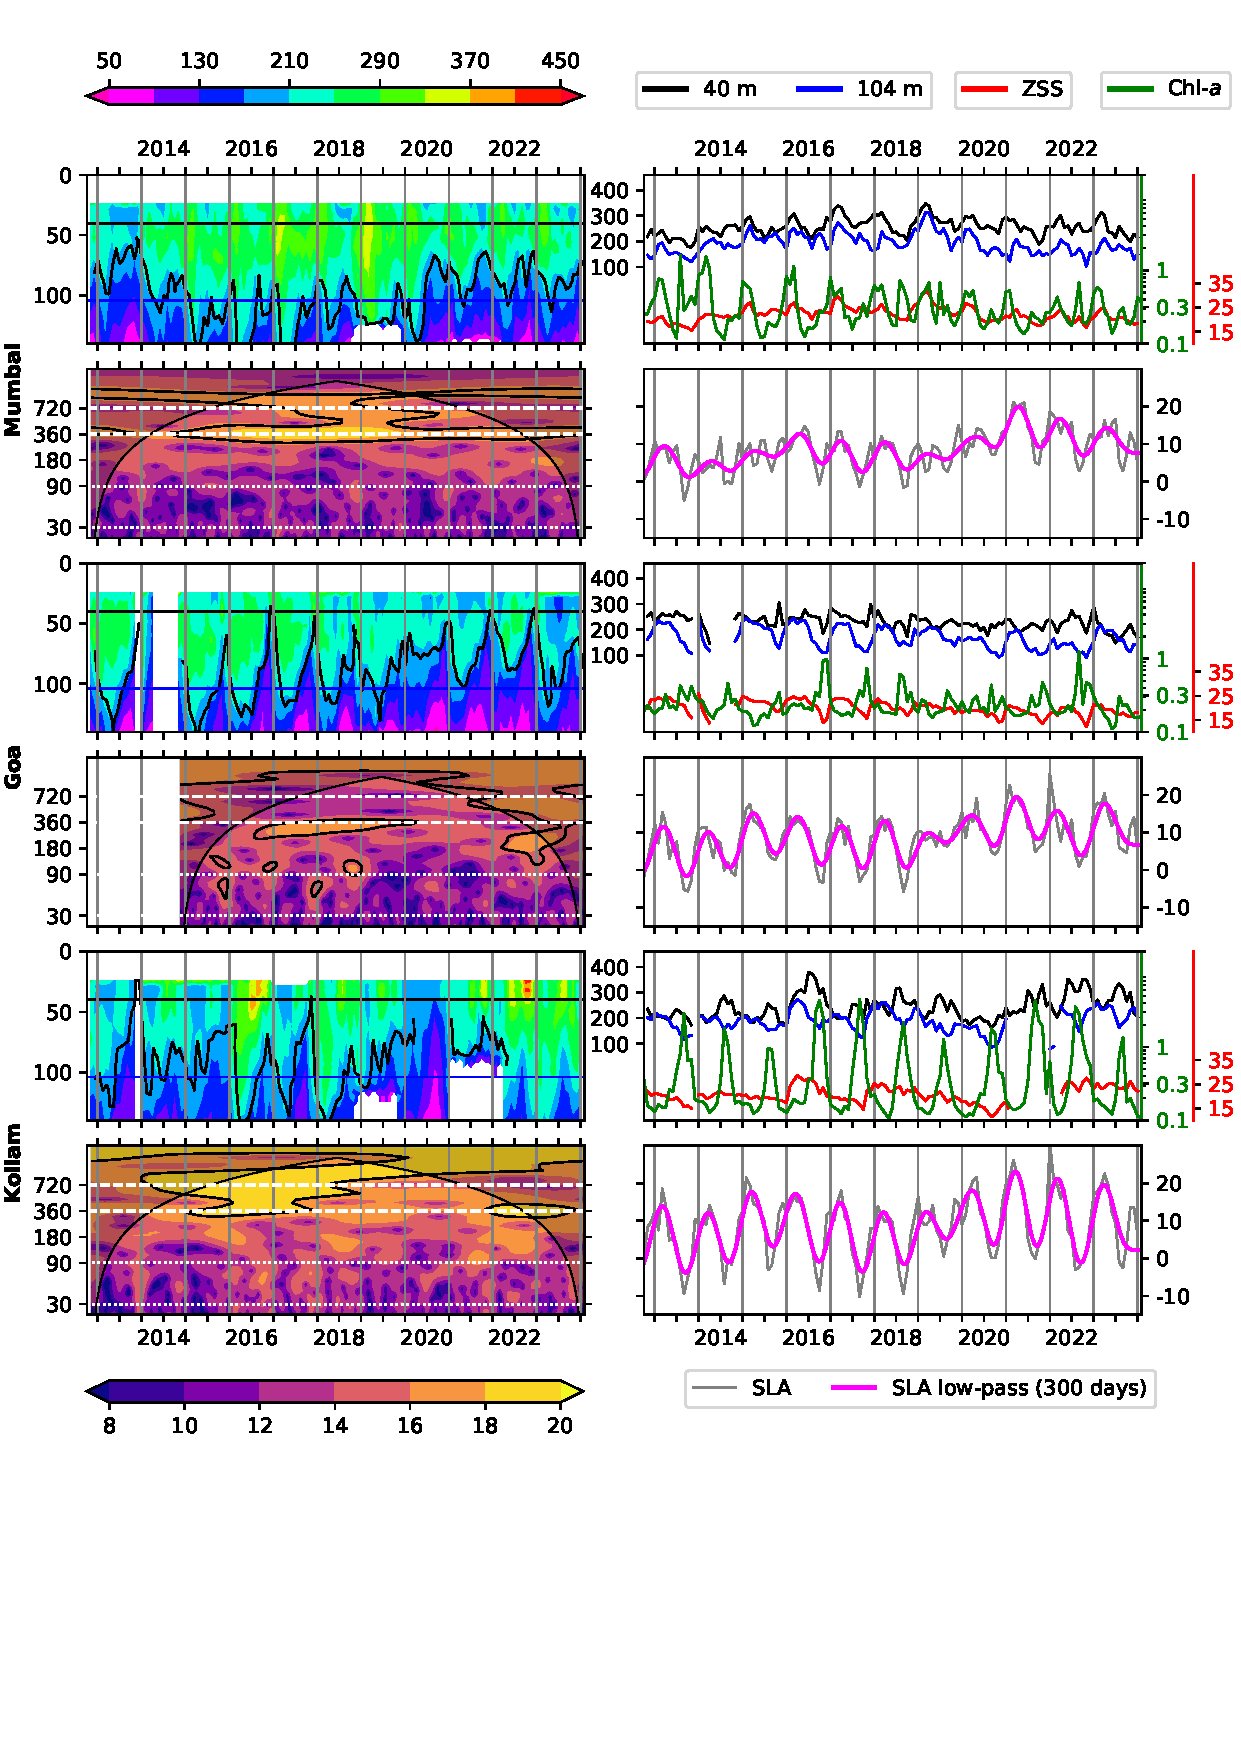
\includegraphics[width=0.95\textwidth]{./figures/biomass_ss_chl.pdf} 
	\captionsetup{justification=justified,font=footnotesize,skip=0.05\baselineskip,width=\textwidth}
	\caption{Decade-long biomass records off Mumbai, Goa, and Kollam are shown in the left panels. Black and blue lines indicate biomass at 40~m and 104~m, respectively; vertical grey lines separate years. Biomass is in units of mg\,m$^{-3}$. Below each record, wavelet power spectra of 40~m biomass are shown, with dashed white lines marking $\sim$720 and 360 days, and dotted lines denoting the intraseasonal band (30--90 days). The right panels show time series of biomass at 40~m (black) and 104~m (blue), alongside ZSS (red) and \chla\ (green) for the respective locations. All time series are resampled to a monthly time axis. Sea level anomaly (SLA, grey) is shown adjacent to the wavelet panels, overlaid with its 300-day low-pass filtered signal (magenta).}
	\label{fig:biomass_ss_chl}
\end{figure}

%\begin{figure}[htbp]
%	\centering
%	\includegraphics[width=\textwidth]{./figures/variability_40m_biomass.pdf} 
%	\captionsetup{justification=justified,font=footnotesize,skip=0.05\baselineskip,width=\textwidth}
%	\caption{Biomass variation in intraseasonal band i.e., 30 to 90 days period is obtained using a lanczos band pass filter. The horizontal black and blue lines is for 40 and 104 m, vertical black lines separate the years and solid magenta curves denotes D215 (D175 off Okha and Kanyakumari) fetched from monthly biomass. The dashed line at 22 m marks the top-depth of first bin i.e, 24 m. Intraseasonal variability is seen throughout the record, and it is coherent along the slope and its magnitude is stronger during August to November. The mean of daily biomass at 40 m is shown in top-right of each panel for respective location.}
%	\label{fig:variability_40m_intraseasonal_vs_seasonal}
%\end{figure}

\begin{figure}[htbp]
	\centering
	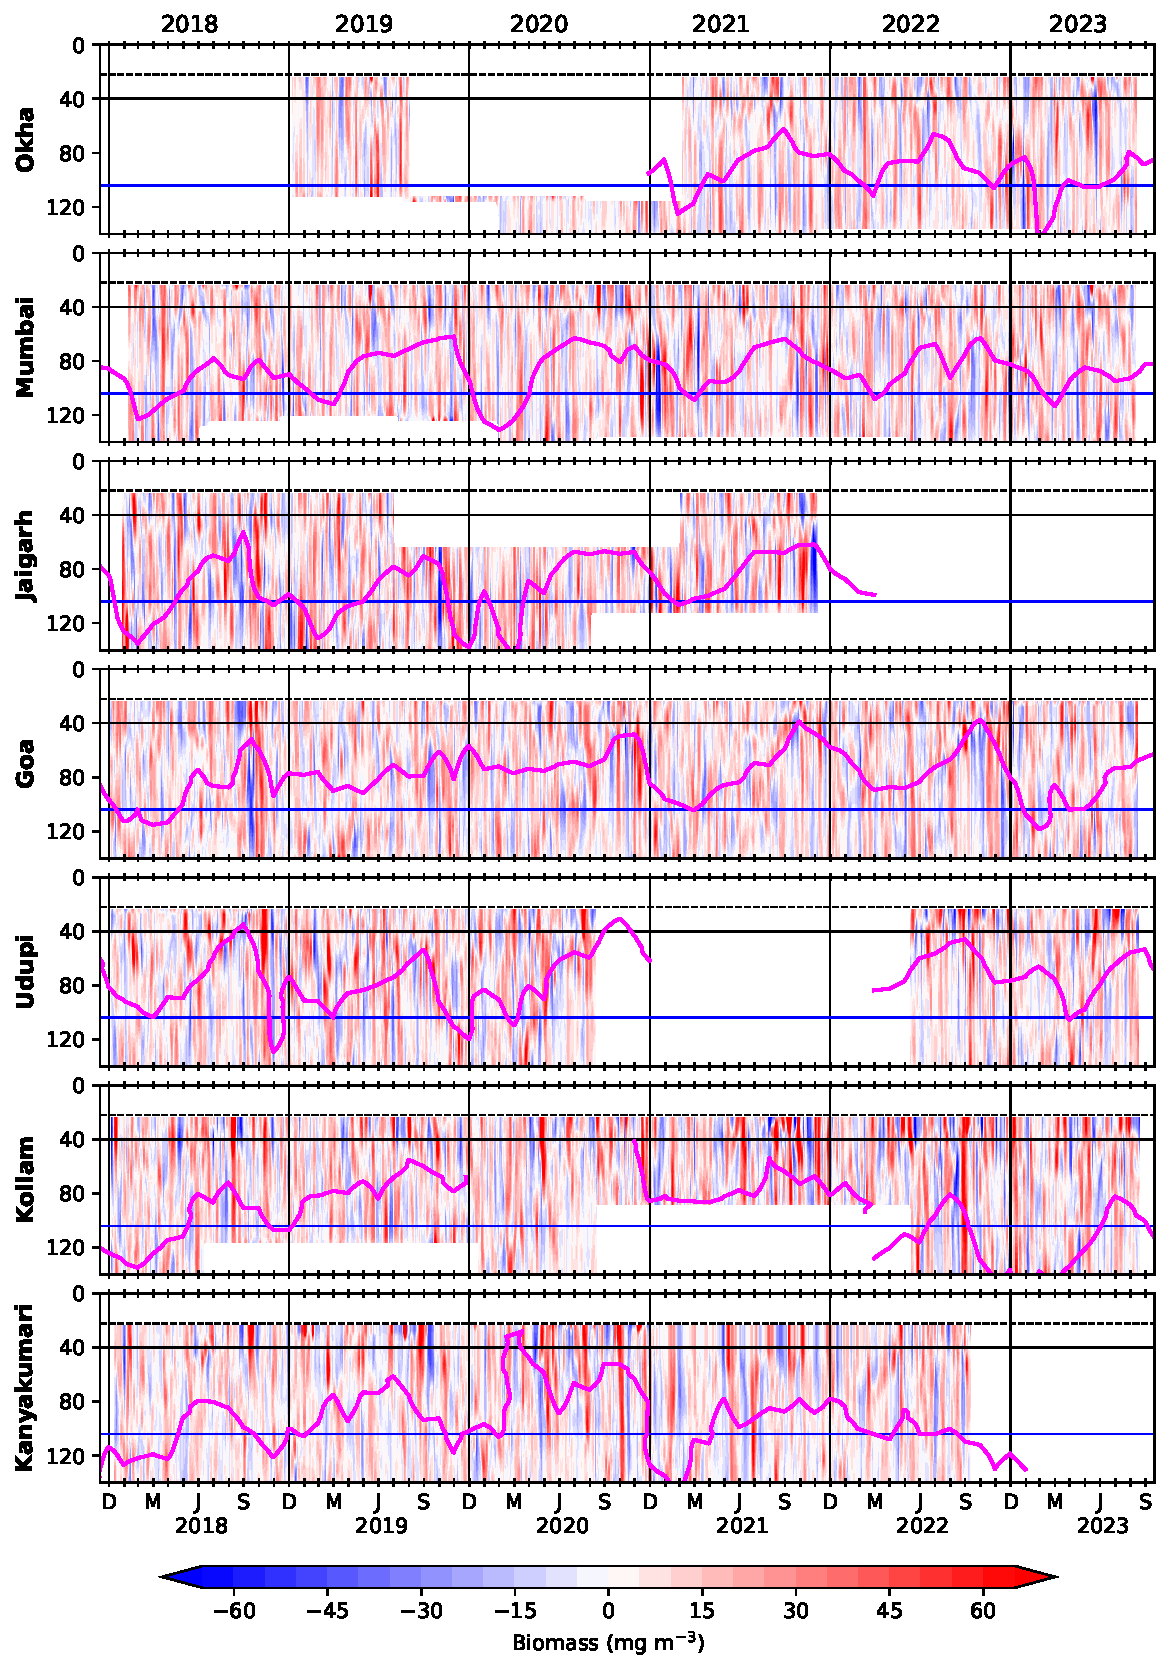
\includegraphics[width=\textwidth]{./figures/filtered_biomass_intraseasonal_5_90days.pdf} 
	\caption{Biomass variation in the intraseasonal band (5--90 day period) is extracted using a Lanczos band-pass filter, capturing both high- and low-frequency intraseasonal components. Horizontal black and blue lines represent depths of 40 m and 104 m, respectively. Vertical black lines separate calendar years, and solid magenta curves indicate $D215$ (or $D175$ off Okha and Kanyakumari), derived from monthly biomass. The dashed line at 22 m marks the upper boundary of the first bin (centered at 24 m). Intraseasonal variability is evident throughout the time series and appears coherent along the slope, notably during October--December 2018.}
	\label{fig:filtered_biomass_intraseasonal_5_90days}
\end{figure}


\begin{figure}[htbp]
	\begin{adjustwidth}{-0.5in}{0in} 
		\centering
		\includegraphics[width=0.9\textwidth]{./figures/biomass_intra_2019_kollam.pdf} 
		\captionsetup{justification=justified,font=footnotesize,skip=0.05\baselineskip,width=\textwidth}
		\caption{Figure consisting multiple plots showing the comparison of biomass variability in the seasonal and intraseasonal bands off Kollam. The top two panels display time--depth plots of seasonal and intraseasonal biomass on the same color scale. D215 is marked in magenta contours, depths of 40 m and 104 m are marked by black and blue lines, respectively, and vertical grey lines indicate month boundaries. The third panel from the top shows daily biomass at 40 m and 104 m, along with its intraseasonal (5--90 days) and seasonal (100--400 days) components. The mean daily biomass for each depth is noted in the bottom right corner of the panel. The fourth panel presents daily biomass overlaid with its 5-day low-pass filtered version and the daily sea level anomaly (SLA). Periods of high (low) SLA are observed to coincide with lower (higher) biomass at 40 m. The fifth panel shows the difference between daily and 5-day low-pass filtered biomass at 40 m and 104 m; grey and light grey shaded regions indicate the 1 standard deviation (SD) and 2 SD envelopes of the backscatter-to-biomass relationship, respectively, over which daily \chla\ is overlaid. The bottom panel presents \chla\ and ZSS in the intraseasonal and seasonal bands. See \textbf{Figs. S4--S9} for a detailed comparison of variability across frequency bands.}		
		\label{fig:biomass_intra_2019_kollam}
	\end{adjustwidth}
\end{figure}


\end{document}
